\section{Understanding the impact of the proposer}
\label{impact}

\subsection{Driving Questions}

Here we focus our attention to understand how proposers with different latencies to other network nodes could impact the overall consensus performance.   When referring to the 'location' of a node in the topology we are here primarily concerned with this aspect.   
Our investigation is driven by the following questions:

\begin{enumerate}[label=(\Roman*)]
    \item Does the location of a proposer have any measurable impact on the consensus? 

    \item Does the location of a proposer affect the duration of individual consensus steps?
    
    \item Does the location of a proposer affect the quorums formed?
    
    \item Can a fixed proposer in an ideal position lead to a better throughput than a rotating approach?  
    
\end{enumerate}


\subsection{Basic Setup}
\label{setup}

To answer these questions, we adopt an experimental approach,
with the following basic setup.
%\addtocounter{footnote}{2}
%\begin{itemize}
    %\item 
    We adopt AWS latencies\footnote{\url{https://github.com/cometbft/cometbft/blob/v2.x/test/e2e/pkg/files/aws-latencies.csv}} as a representative wide-area topology, emulated via tc\footnote{https://www.man7.org/linux/man-pages/man8/tc.8.html}. 
    %\item 
    One consensus participant node per AWS zone is deployed, i.e. 13 nodes. 
    %\item 
    Within CloudLab\footnote{\url{https://cloudlab.us/}}, we use m510\footnote{\url{https://docs.cloudlab.us/hardware.html\#(part.cloudlab-utah)}}  nodes configured to share a local network.
    % 
    %\item we multiply latencies uniformly to ensure run-to-run repeatability, which can be necessary during periods of high external load to reduce the effects variability in the underlying network have in our emulated topologies (the focus of our study). In such cases we also increase the timeouts to ensure constant 1 round consensus; 
    %
    %we multiply latency and timeouts as needed to ensure constant 1 round consensus and run-to-run repeatability\footnote{CloudLab sporadically exhibits low-amplitude network noise due to high external load. In configurations with low emulated latencies, this noise becomes proportionally significant and introduces non-negligible network variability across runs. As our objective is to study the given topologies, and not the underlying physical structure, we apply a uniform scaling factor to all latencies. This preserves the relative topology while reducing the relative impact of external noise, improving repeatability. When compared with the original, unscaled topology, quorum formation remains unchanged and consensus time and throughput scales proportionally.};  
    %\item 
    Executions last 5 minutes (including 30 seconds warm-up and 15 seconds of cool-down at the end), each setup is repeated at least once to ensure consistent results.
    %\item 
    We employ the latest version of Malachite Starknet (v0.4.x) as our implementation of Tendermint, instantiated according to the QA system\footnote{\url{https://github.com/circlefin/malachite/tree/greg/qa-fix-write/qa}}.
    %\item 
    Nodes are synchronized with NTP \footnote{\url{https://www.ntp.org/}} to ensure less than 10ms of deviation between clocks. 
    %Synchronization does not affect the experiments in any way but facilitates the calculation of some of our metrics. 
%\end{itemize}

%The complete latency matrix and complementary node specifications are provided in Appendices \ref{awslat} and \ref{apdex}, respectively.

\subsection{Fixed vs. rotating proposer}
We start with a sanity check to evaluate whether the performance of rotating proposers is equivalent to fixed proposers in our setup. We configure a 4-node topology with uniform 100ms latency between all pairs, with remaining parameters following the basic setup. We run two executions with the default rotating proposer and two executions with each node acting as a fixed proposer, each execution producing around 450 blocks.  We measure block time at the proposer (time from the start of propose step to end of decided step), and report the mean block time duration, 80th percentile, and 90th percentile.  We then compute the maximum absolute difference for each metric across all runs and configurations. The resulting maximum differences are: 0.6\% for the 80th percentile, 1.6\% for the 90th percentile, and 1.1\% for the mean.  {\it With this, we consider fixed and rotating proposer as having equivalent performance with uniform network latencies.} 

%- and negligible relative to the effects observed in the subsequent experiments. 


\subsection{Proposer location impact on consensus latency - Question I}
%\begin{itemize}
%    \item Does the location of a proposer have any measurable impact on the consensus?
%\end{itemize}

Next, we conduct experiments using the basic setup (i.e. with emulated AWS latencies) to measure the impact of proposer location in a topology with heterogeneous latencies.  To ease visualization, we show results with a a modified version that rotates every 10 decisions\footnote{The performance is equivalent to the original version which rotates the proposer after every decision.}
%
%We run experiments with both the default proposer rotation algorithm, which rotates the proposer after every decision, and with a modified version that rotates every 10 decisions. The two algorithms are functionally equivalent and show  no observable differences across all measured metrics.  However, as the 10x algorithm effectively lengthens the patterns caused by individual proposers, these patterns are easier to observe in the corresponding graphs. For readability, we only show the 10x results below. 

Figure \ref{Idur} plots the results, measuring consensus time (proposal to decision) at the proposer. Proposer changes are marked by vertical purple dotted lines, with a solid vertical mark denoting a rotation back to the first proposer. 
%
Certain proposers consistently lead to faster or slower decisions relative to the average, repeating the pattern as they are elected again, indicating that these differences are not due to external transient factors.   
Considering the results of our first experiment with uniform latencies and that the only different aspect to this second experiment are the heterogeneous latencies, we 
attribute the different performance of proposers exclusively to their position 
in the topology.  Consensus duration ranges from $0.47s$ to $0.73s$, with a mean of $0.54s$ and a standard deviation of $0.05$, showing that {\it the position of the proposer can drastically affect the duration of consensus} (and therefore the throughput of the system) even in a proposer-based consensus. 

Figure \ref{Idev} gathers the same information across the system, measuring time from the proposer's proposal to the decision of every node. A vertical line refers to a consensus instance.  Its width (or darkness) varies with the vertical axis, being proportional to how many nodes had that latency to terminate that consensus instance.  We also plot the system average latency (red) and the per-instance latency (yellow).
%
We identify patterns related to the proposer, showing that the {\it proposer choice affects the consensus termination latency at every single node in the network}, and not just its local view.  Therefore, we conclude that the overall performance depends not only on network topology but also on the proposers’ positions within that topology.


\begin{figure}[htbp]
\centerline{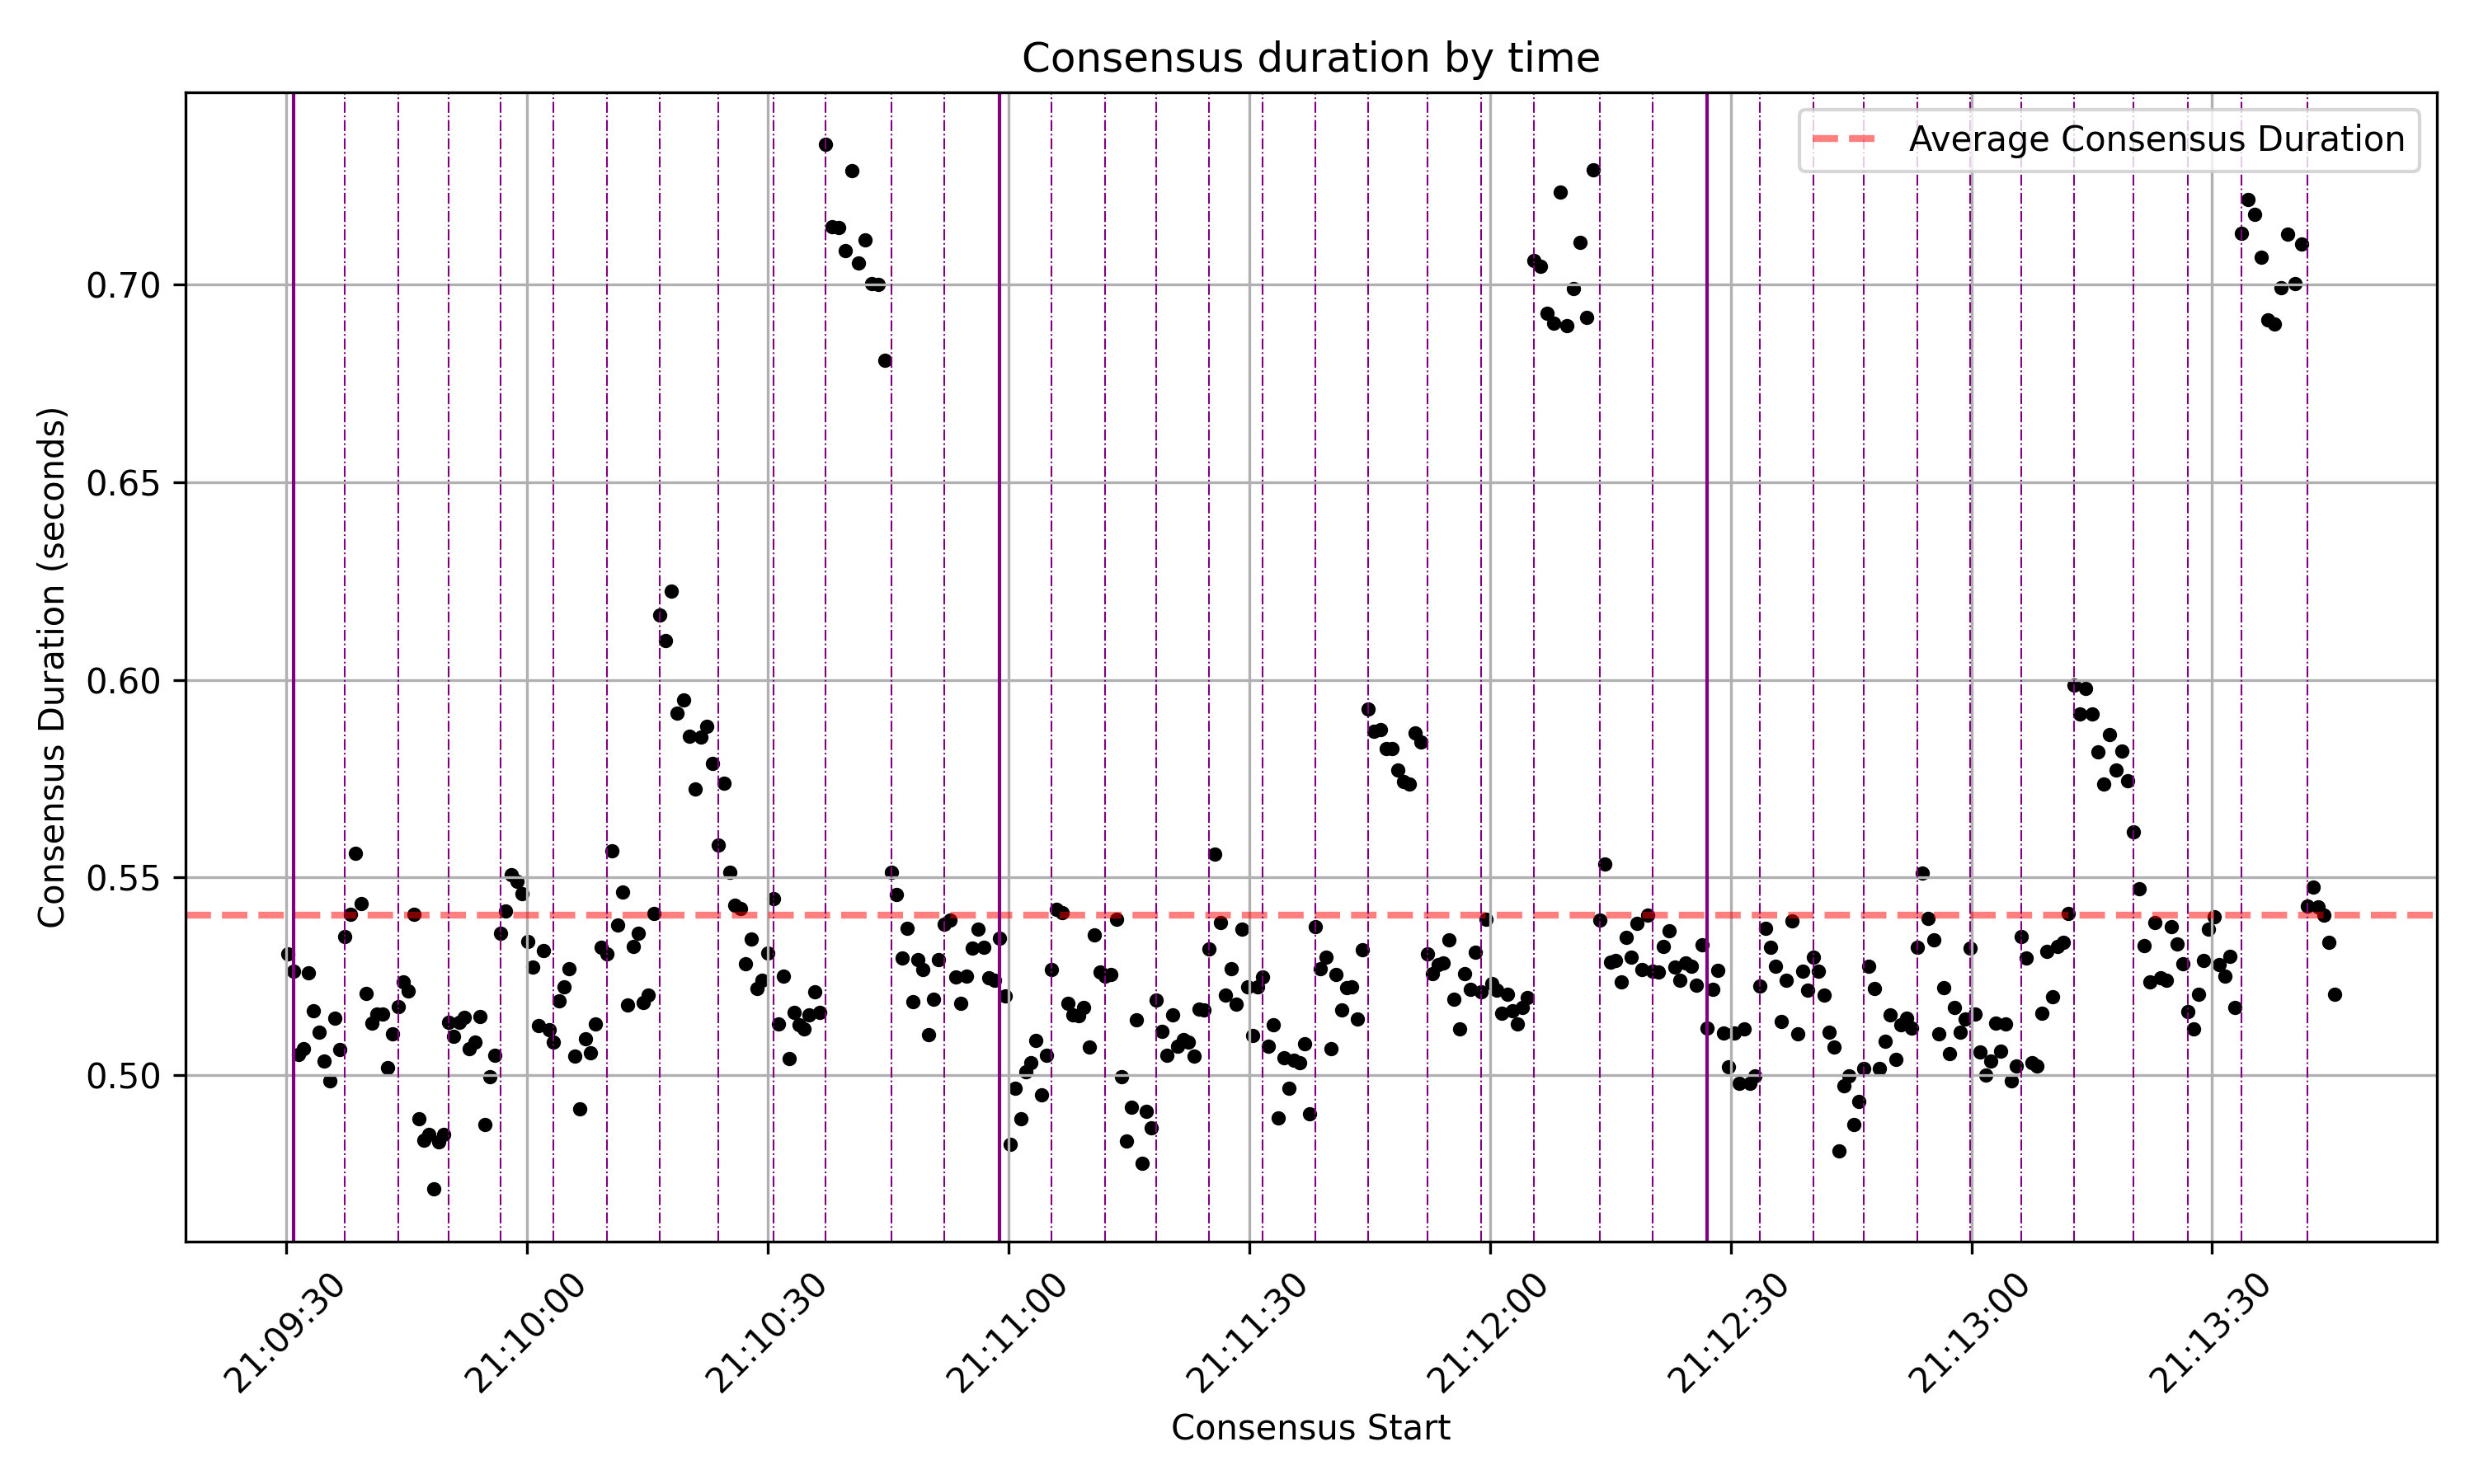
\includegraphics[width=0.39\textwidth]{img/10xconsensusDuration.png}}
\caption{Consensus durations (10x proposer)}
\label{Idur}
\end{figure}


\begin{figure}[htbp]
\centerline{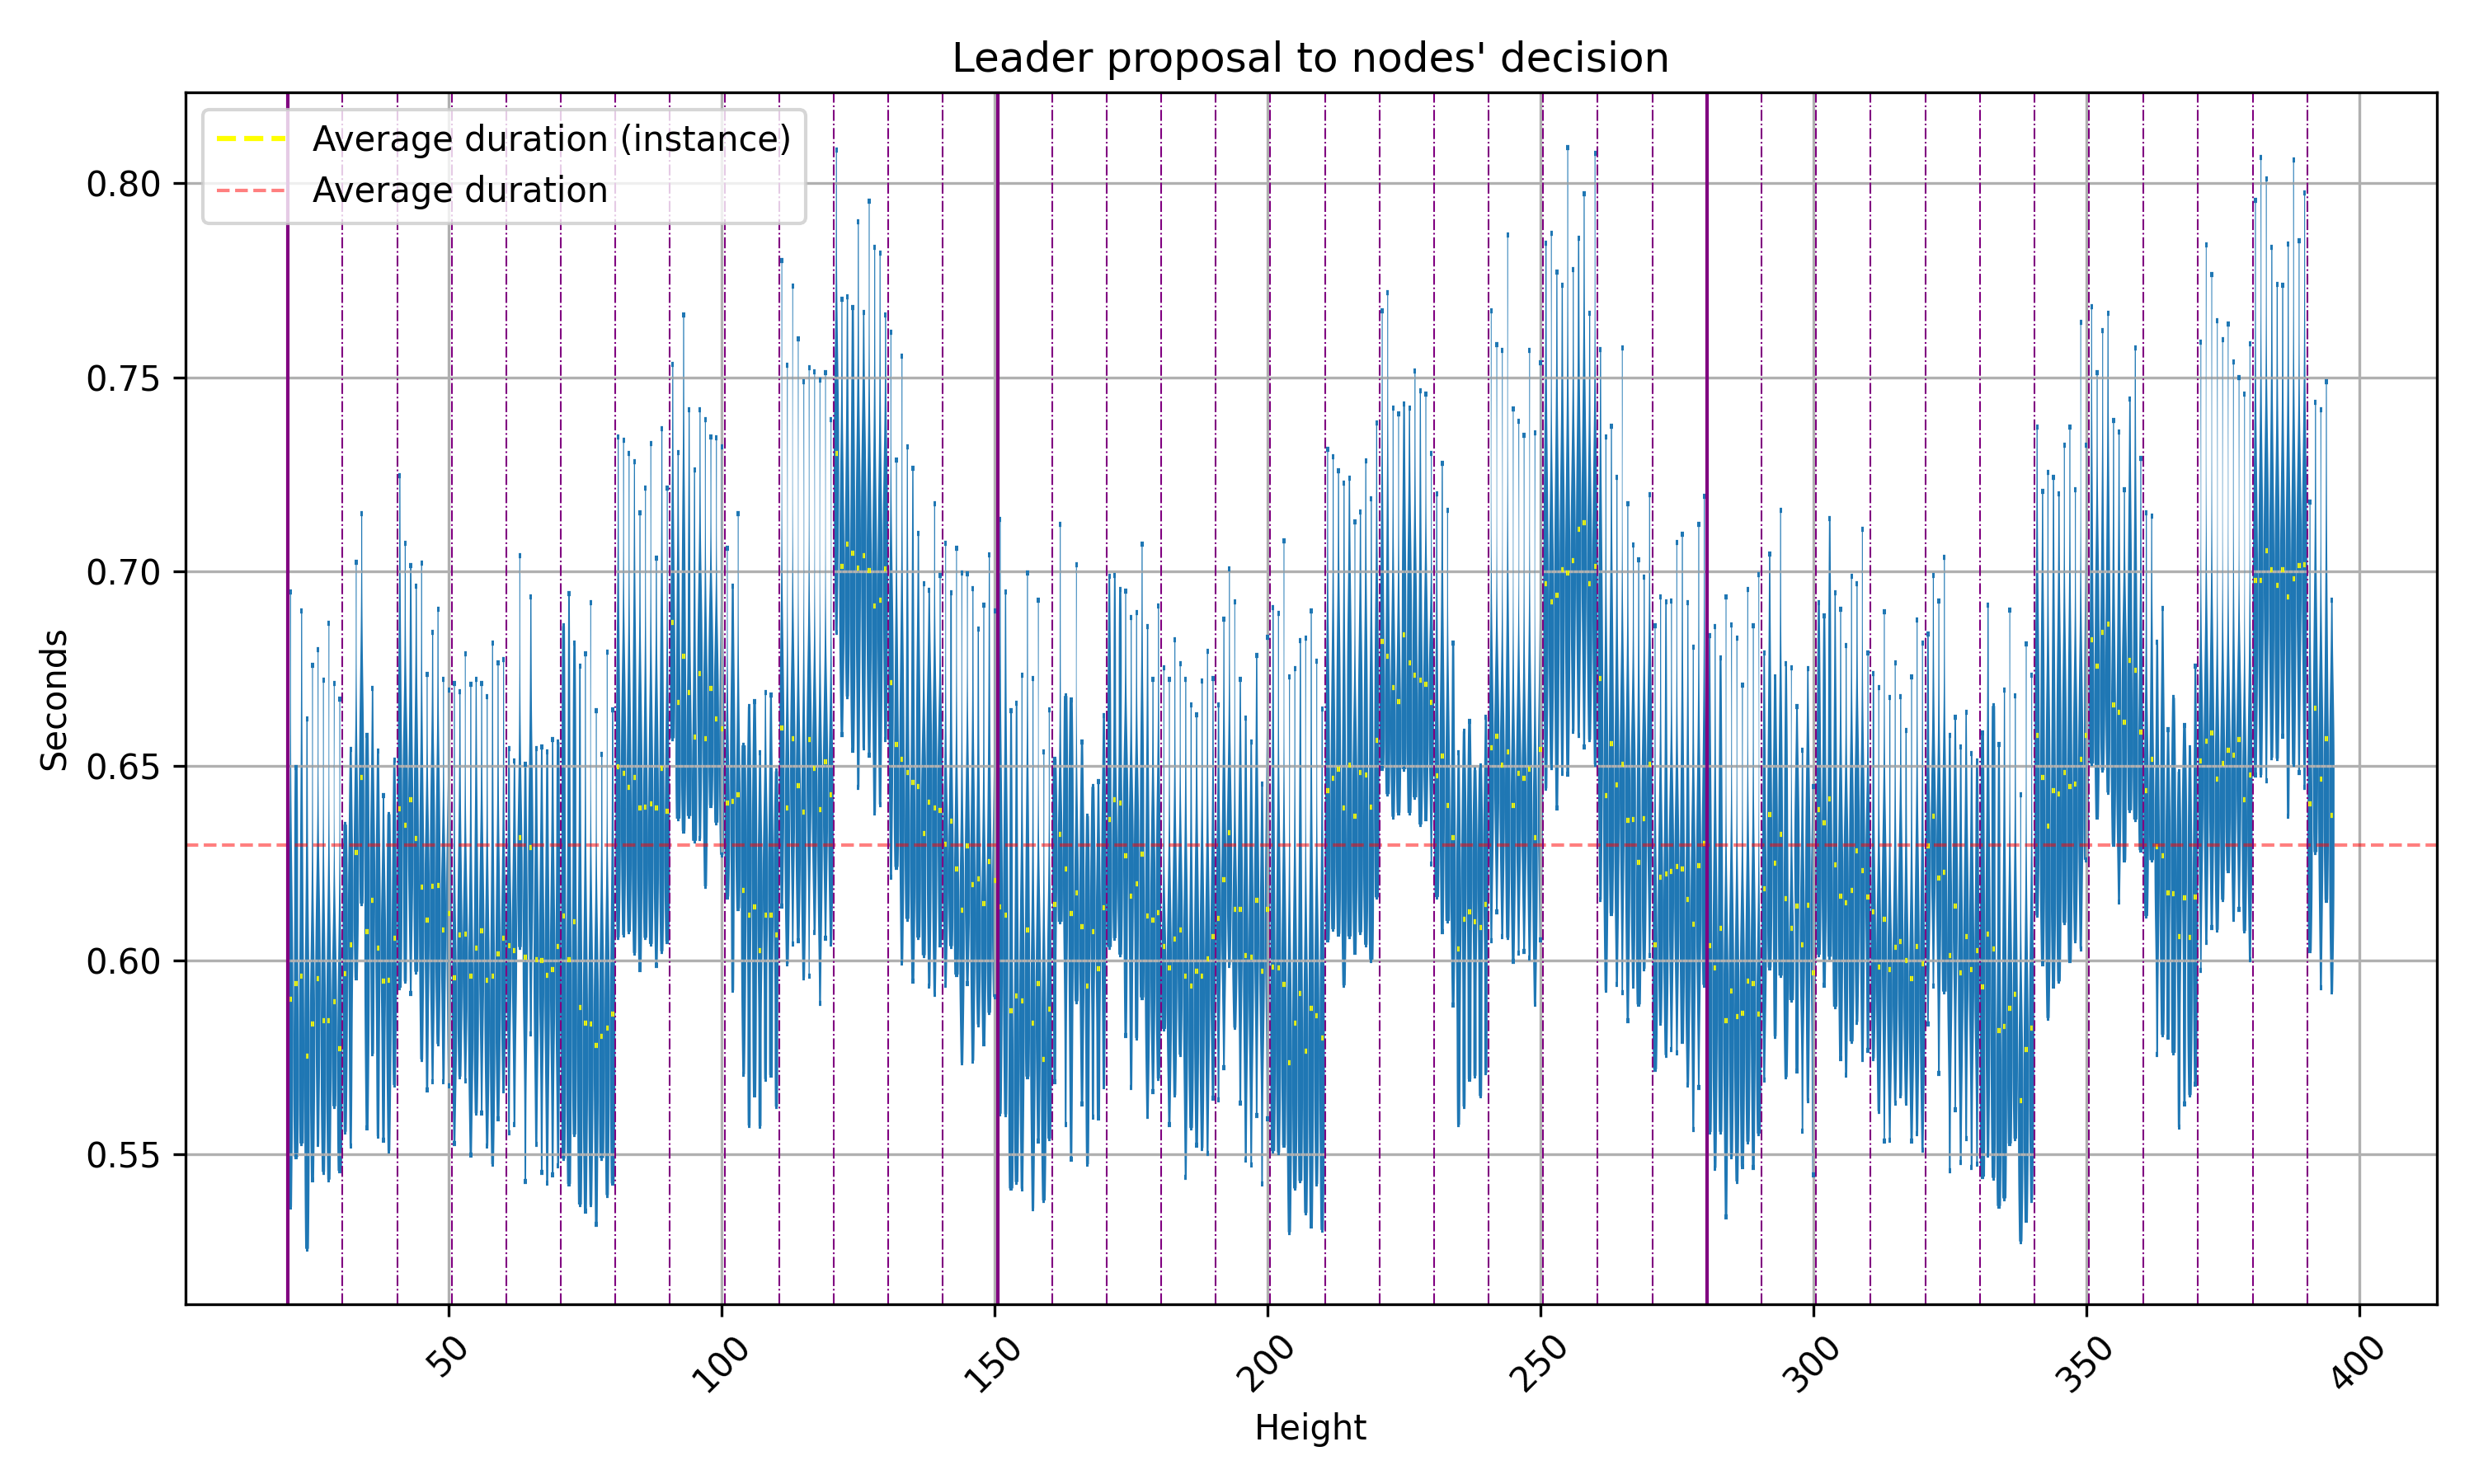
\includegraphics[width=0.4\textwidth]{img/10xdecidedDeviationBlocktime.png}}
\caption{Decided deviation (10x proposer)}
\label{Idev}
\end{figure}




\subsection{Proposer location impact on duration of consensus steps -Question II}
%\begin{itemize}
%    \item Does the location of a proposer impact the duration of individual consensus steps?
%\end{itemize}

In a proposer based algorithm, the position of the proposer is assumed not to matter past the first consensus step (proposal) since the following steps are all symmetric (from all to all) across nodes.
To verify whether the impact was limited to the proposal step, we measured and compared the duration of the following steps (prevote and precommit) across the network. 

Fig \ref{II} shows the duration of the prevote step and the prevote and precommit steps combined, measured at each node in the network.  The prevote duration is defined as the time elapsed from receiving a proposal until a quorum of prevotes is received. The precommit duration is defined as the time elapsed from the moment a node receives a quorum of prevotes until a quorum of precommits is received.

We compute the local duration of each step at each node and show the network mean (vertical blue line) of each consensus instance, as well as the per-proposer mean (green line). 


While individual steps are often brief and more sensitive to variations in computation time or message delivery, there still emerge clean repeating patterns where certain proposers consistently cause consensus to be faster or slower than average, being similar to the previous patterns in the prevote figure. 


\begin{figure}[htbp]
\centerline{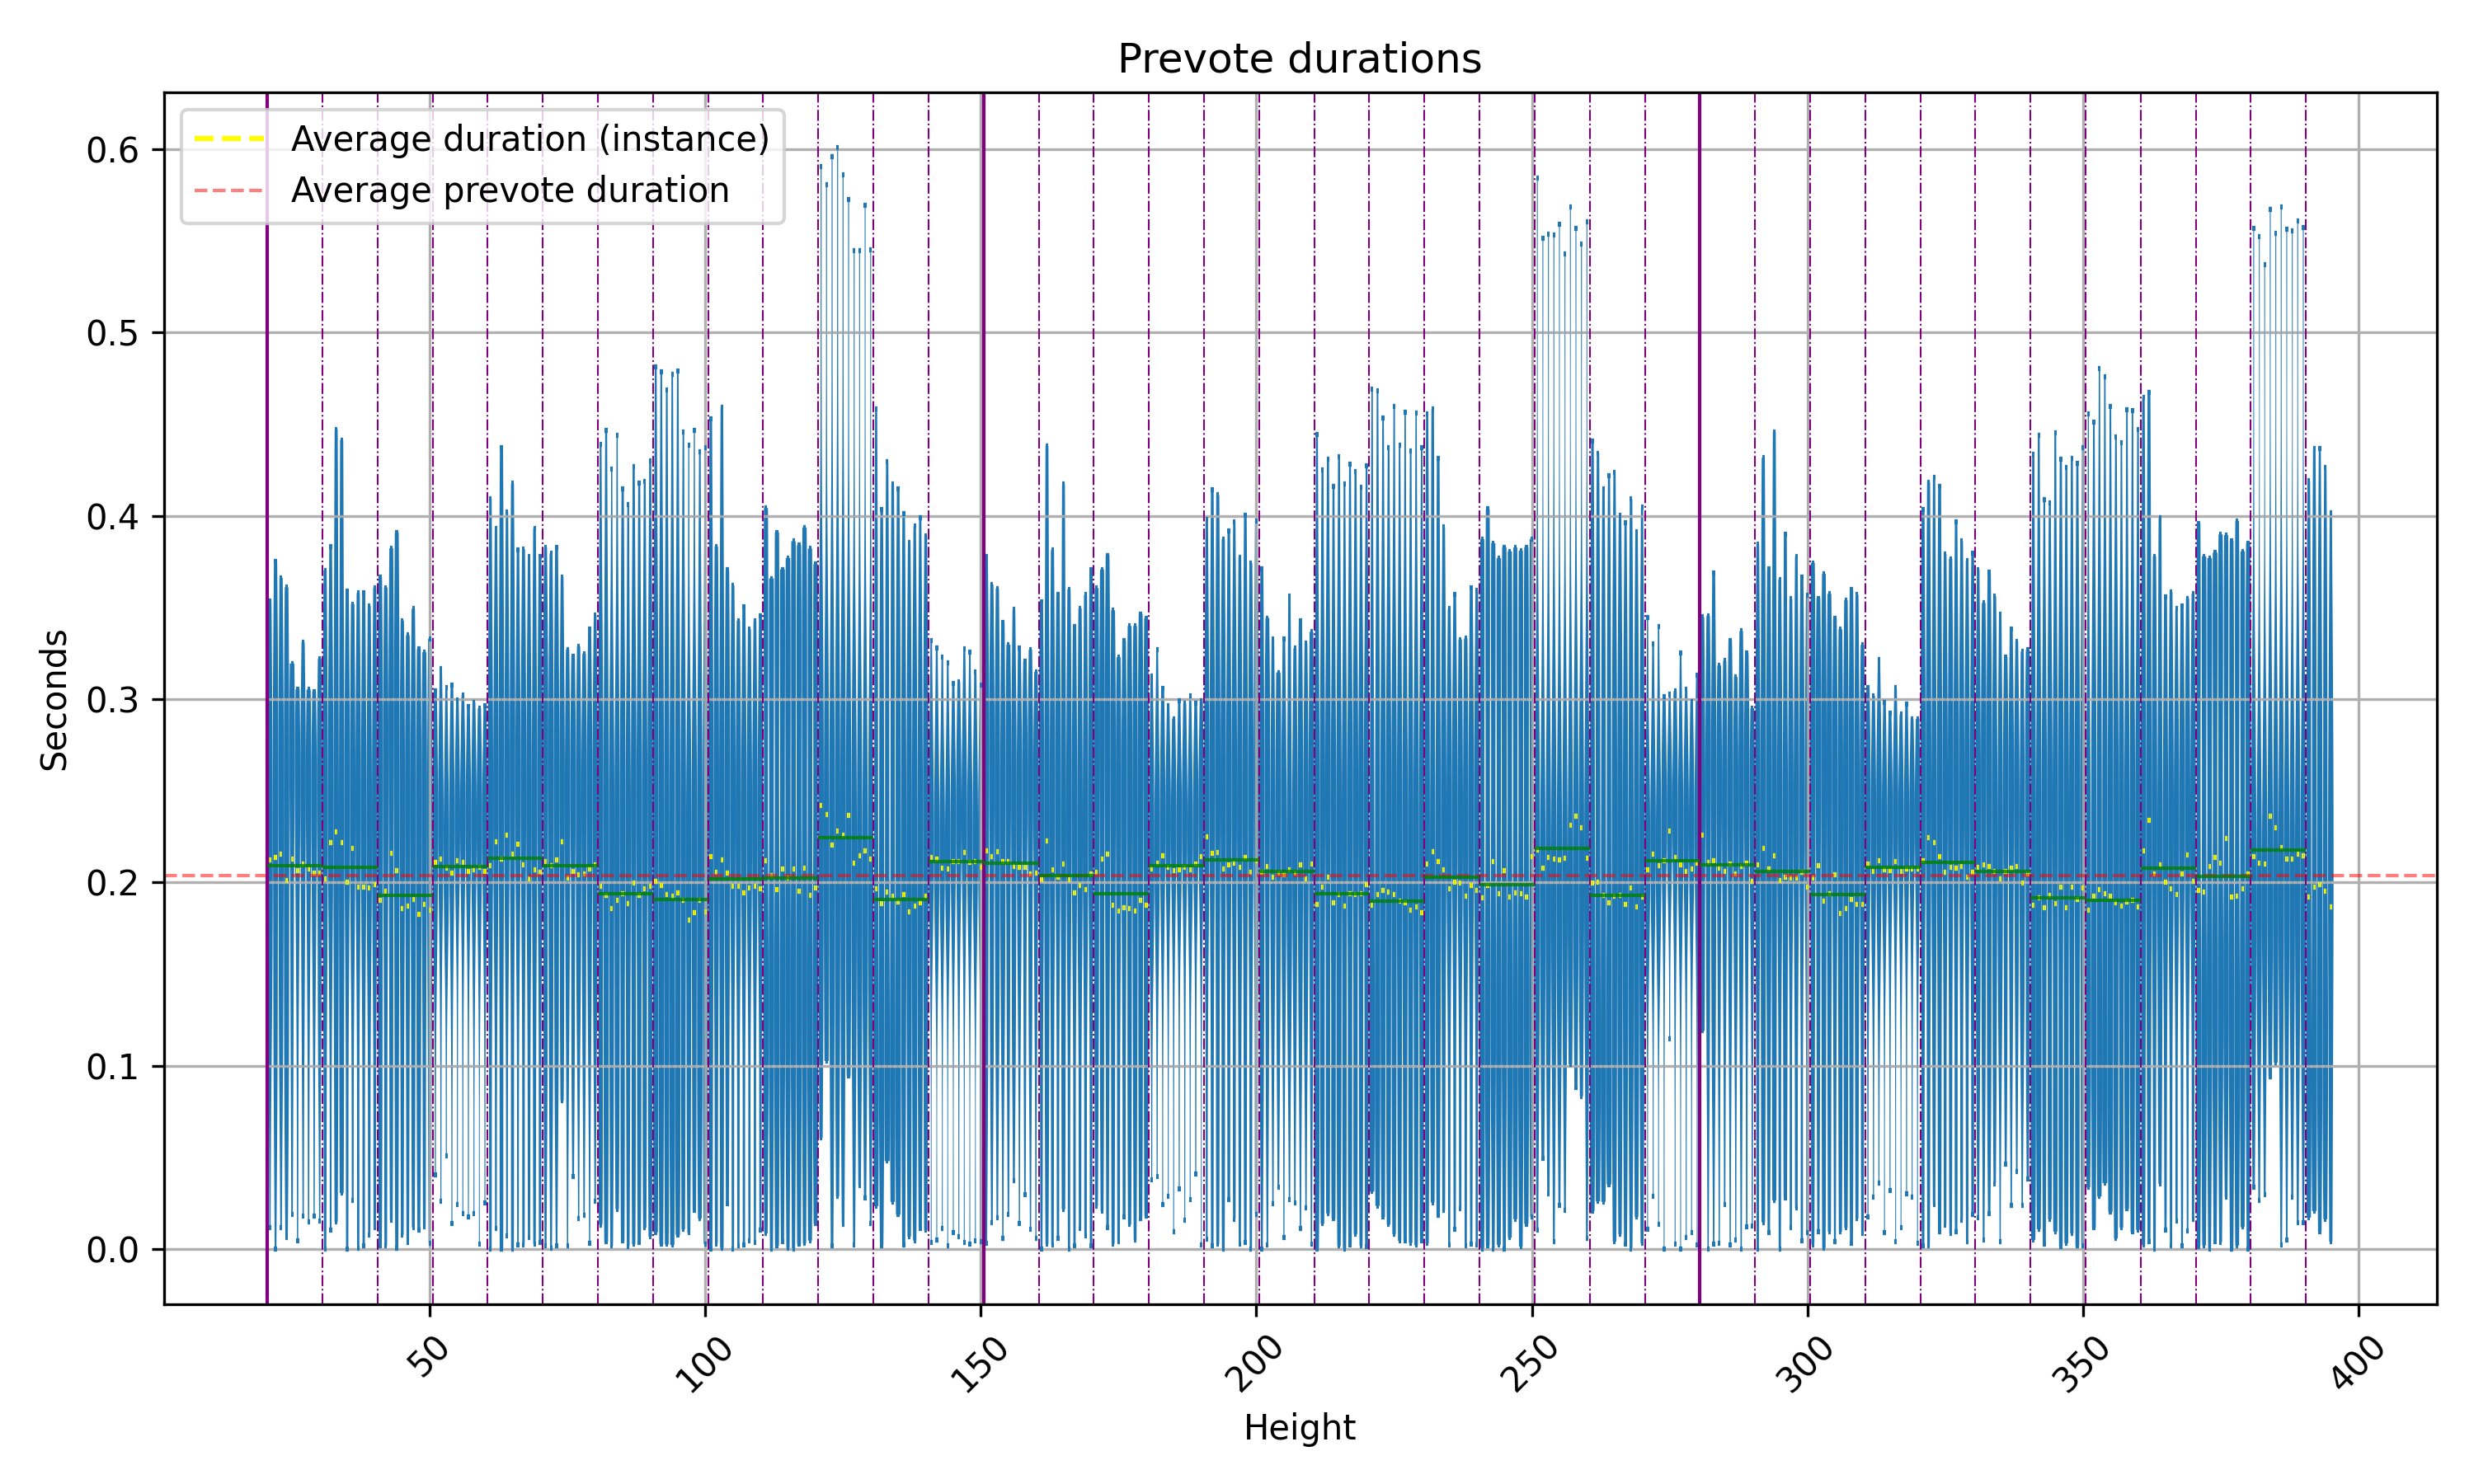
\includegraphics[width=0.39\textwidth]{img/10xstepPrevote.png}}
\centerline{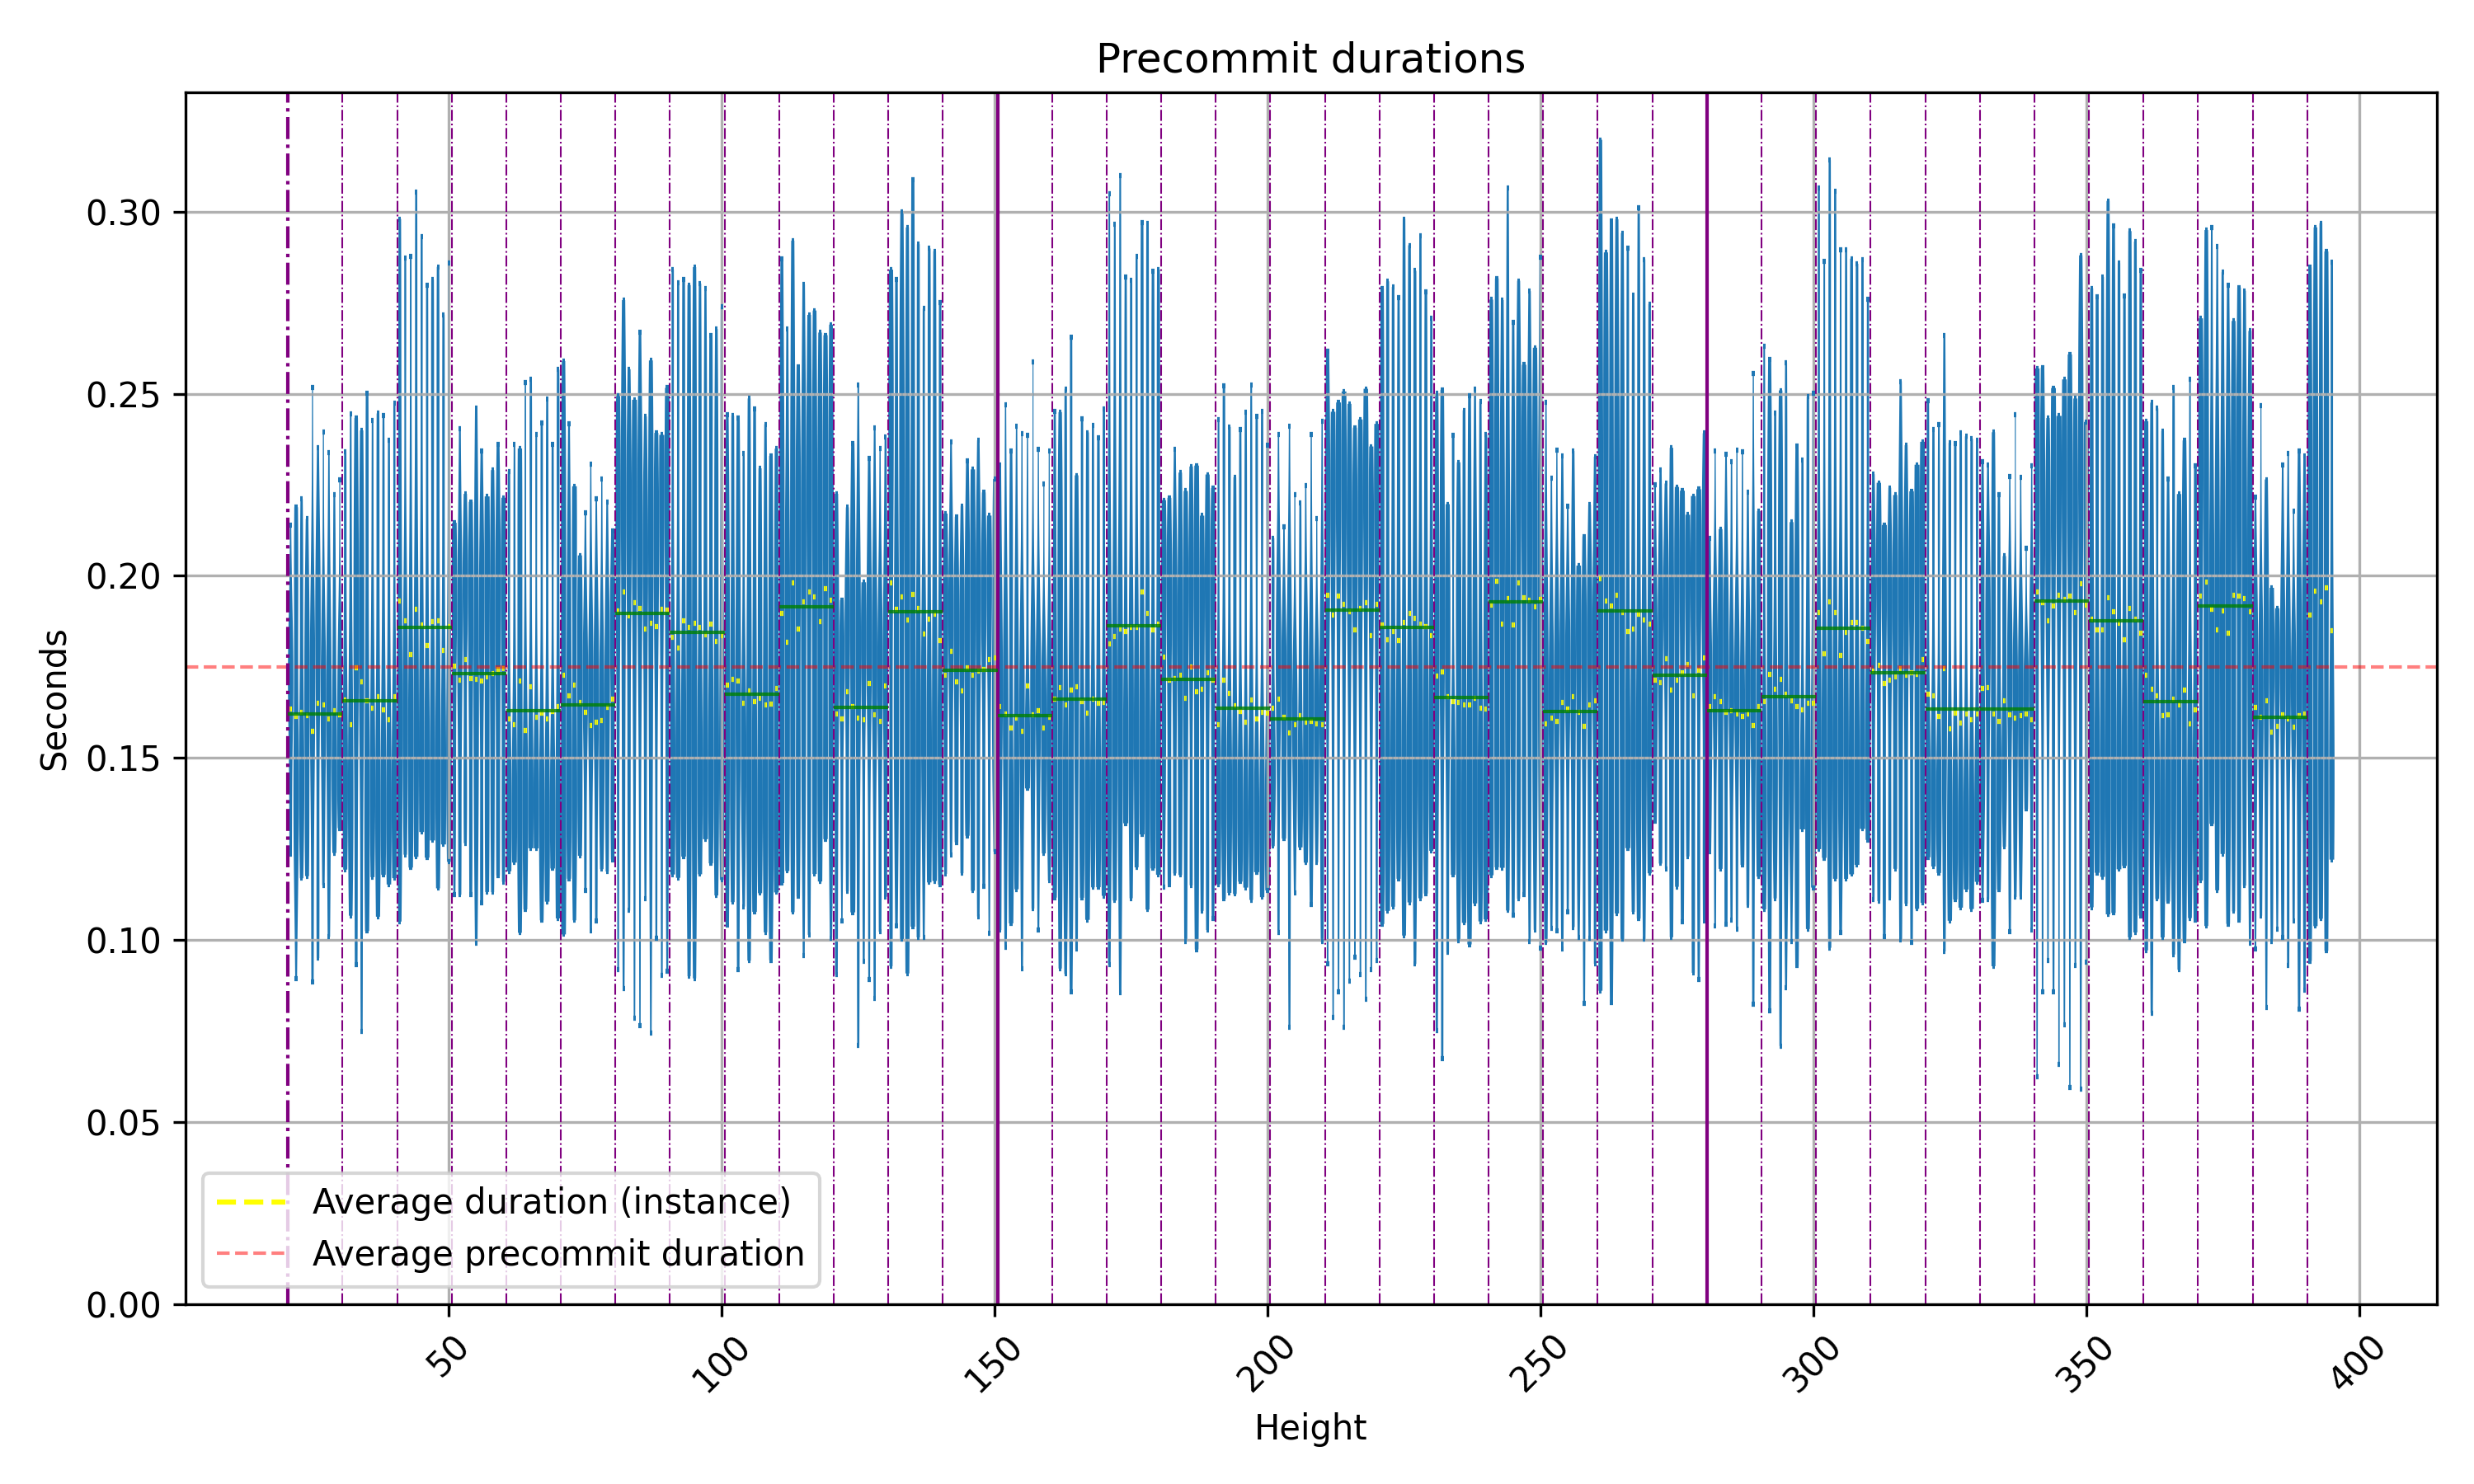
\includegraphics[width=0.39\textwidth]{img/10xstepPrecommit.png}}
\caption{Prevote (top) and prevote plus precommit (bottom) durations (10x proposer)}
\label{II}
\end{figure}

This shows that the location of a proposer also measurably affects the latency of each step, leading into the next question.

\subsection{Question III}
\begin{itemize}
    \item Does the location of a proposer impact the quorums formed?
\end{itemize}

In proposer-based consensus, the position of a proposer is generally assumed not to impact the system beyond the proposal step. If the proposer is disproportionately far from the rest of the system, or if it crashes after the proposal, the remainder of the system is able to continue the consensus unaffected. However, as shown in the previous section, the position of the proposer does affect prevote and precommit durations. One possibility is that the proposer affects the formation of quorums, which in turn affects step durations. To evaluate this hypothesis we look into quorum formation across two sequential network-wide rotations. 


\begin{figure*}[!t]
\centerline{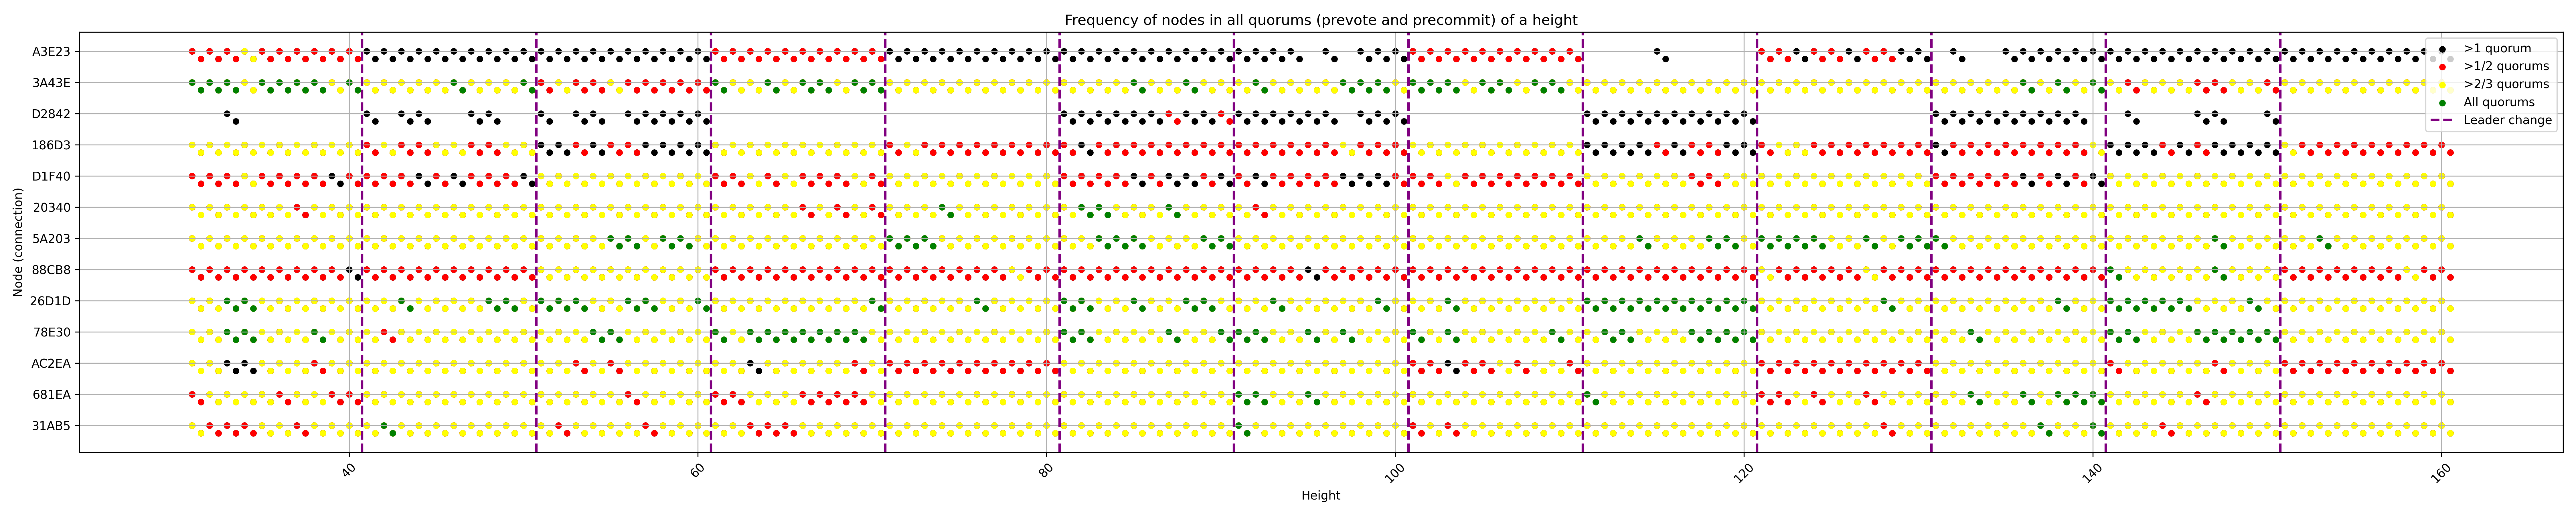
\includegraphics[width=\textwidth]{img/quorum30-160.png}}
\caption{Frequency of nodes in quorums (Height 30-159)}
\label{IIIq1}
\end{figure*}

\begin{figure*}[!t]
\centerline{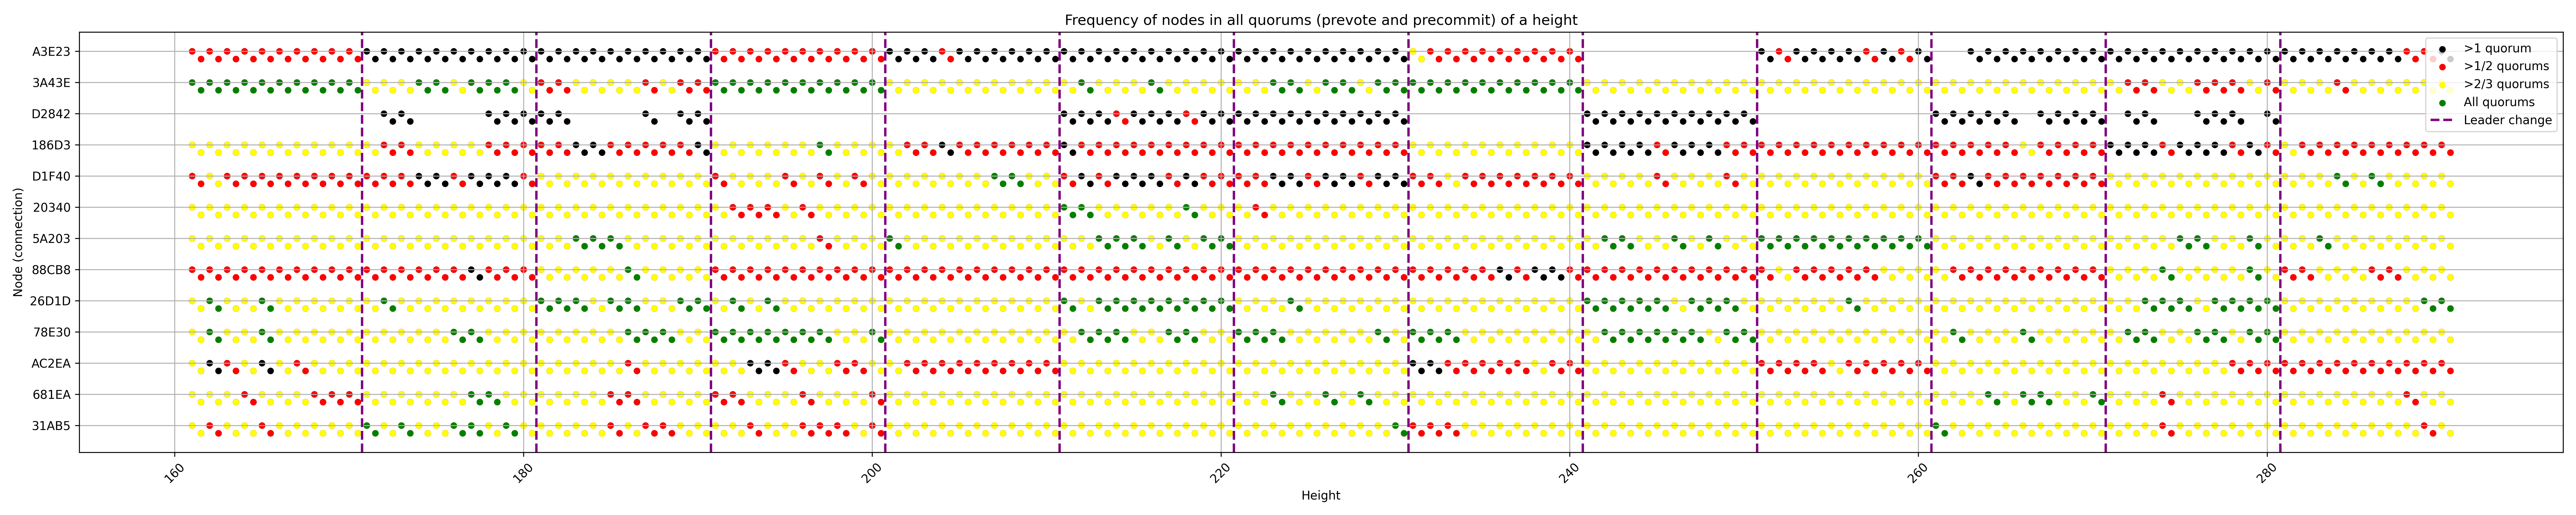
\includegraphics[width=\textwidth]{img/quorum160-290.png}}
\caption{Frequency of nodes in quorums (Height 160-289)}
\label{IIIq2}
\end{figure*}

Fig \ref{IIIq1} and Fig \ref{IIIq2} show the same sequence of proposers one rotation apart. In these graphs the color of each dot represents its frequency in the quorums of other nodes. If a node is only present in its own quorum it does not get drawn on the graph; if it appears in at least one other node it's drawn as a black dot; and so on. Each dot on a line represents the node's frequency on a prevote quorum, with its respective precommit quorum being dislocated down and to the right for readability. As in the previous figures, each node serves as the proposer for 10 consecutive instances before rotating to the next (represented by the purple line). 

These graphs show two important factors that contribute to the speed of the consensus. 
First, as stated in the Tendermint specification, if a farther node manages to join another node's prevote quorum, that second node will wait for that node in the precommit step even if a faster quorum is reached\footnote{This is intended for Proof of Stake rewards.}. 
An effect of this can be seen in the graph where every prevote frequency repeats in the precommit frequency of that height.
If a proposer causes a distant node to join an otherwise ideal prevote quorum, nodes will then be forced to wait for that distant node in the precommit quorum (up to a timeout). This propagates delays across steps. 

And second, there are clear patterns that appear within the frequency of each node relative to which node is the proposer. Between these two graphs there is a 98\% overlap between the frequency of nodes within the periods of each leader. This indicates that the location of the proposer does in fact affect quorum formation.
% Some  nodes consistently exhibit a certain frequency with some proposers, and consistently exhibit other frequencies with other proposers. 
%Putting these two factors together we can understand the impact of the proposer as also affecting which quorums form, and if a slower node happens to be included in a quorum it will propagate to the precommit step, thus slowing the consensus.
%
%\begin{figure}[htbp]
%\centerline{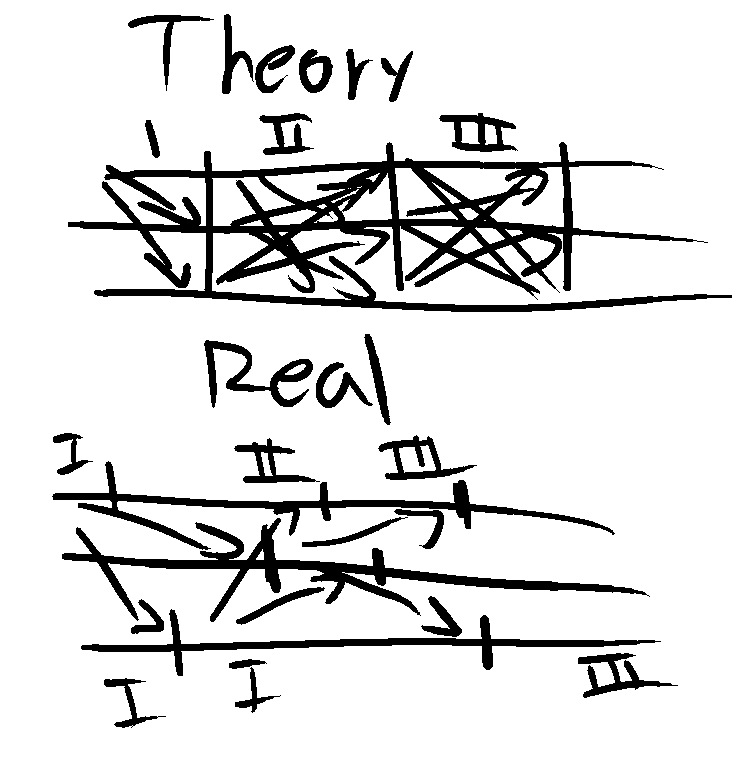
\includegraphics[width=0.3\textwidth]{img/steps.png}}
%\caption{Simplified vs real step change in a topology}
%\label{IIIsteps}
%\end{figure}
%
%That second factor can be understood intuitively by separating the simplified phase change diagram from its real representation (Fig \ref{IIIsteps}). In a system with heterogeneous network latencies nodes will receive the same messages at different times, and this means that nodes are unlikely to enter the same step at the exact same time. 
%
%\fd{este texto parece um pouco alongado e repetitivo.  o trecho a seguir parece sintetizar a ideia e acho que algumas partes acima podem ser suprimidas}
Even if there is an ideal quorum which decrease consensus latency, the existence of that quorum relies on the positioning of the proposer. If the proposer is closer to nodes outside of the ideal quorum, those nodes will receive the proposal first, send their prevote messages first, and therefore be more likely to participate in other quorums, negatively impacting consensus latency and throughput. 

With this information we can now re-examine the previous question with quorum formation in mind. If we relate the step durations in Figure \ref{II} to Figure \ref{Idev} we can see that the corelation isn't perfect. This can be explained by treating quorum formation and proposal latency as two separate factors. A proposer may be topologically distant, and thus imply in non-negligible latency in the initial proposal that slows its consensus speed, but reach nodes in a way that benefits quorum formation and therefore cause the prevote and precommit steps to be faster than average. This illustrates the complexity that topologies can have even on consensus across homogeneous hardware. 


\subsection{Question IV}
\begin{itemize}
    \item Can a fixed proposer in an ideal position lead to a better throughput?
\end{itemize}

So far we have analyzed the theoretical impact of a proposer's location by extrapolating its impact from observations within a rotative system. It is entirely possible that reducing the number of proposers, or increasing their frequency, could increase the computational load of each proposer and impact its performance. To account for those factors we ran experiments comparing the extremes (one single node as the permanent proposer) with the default rotative system. 


\begin{figure}[htbp]
\centerline{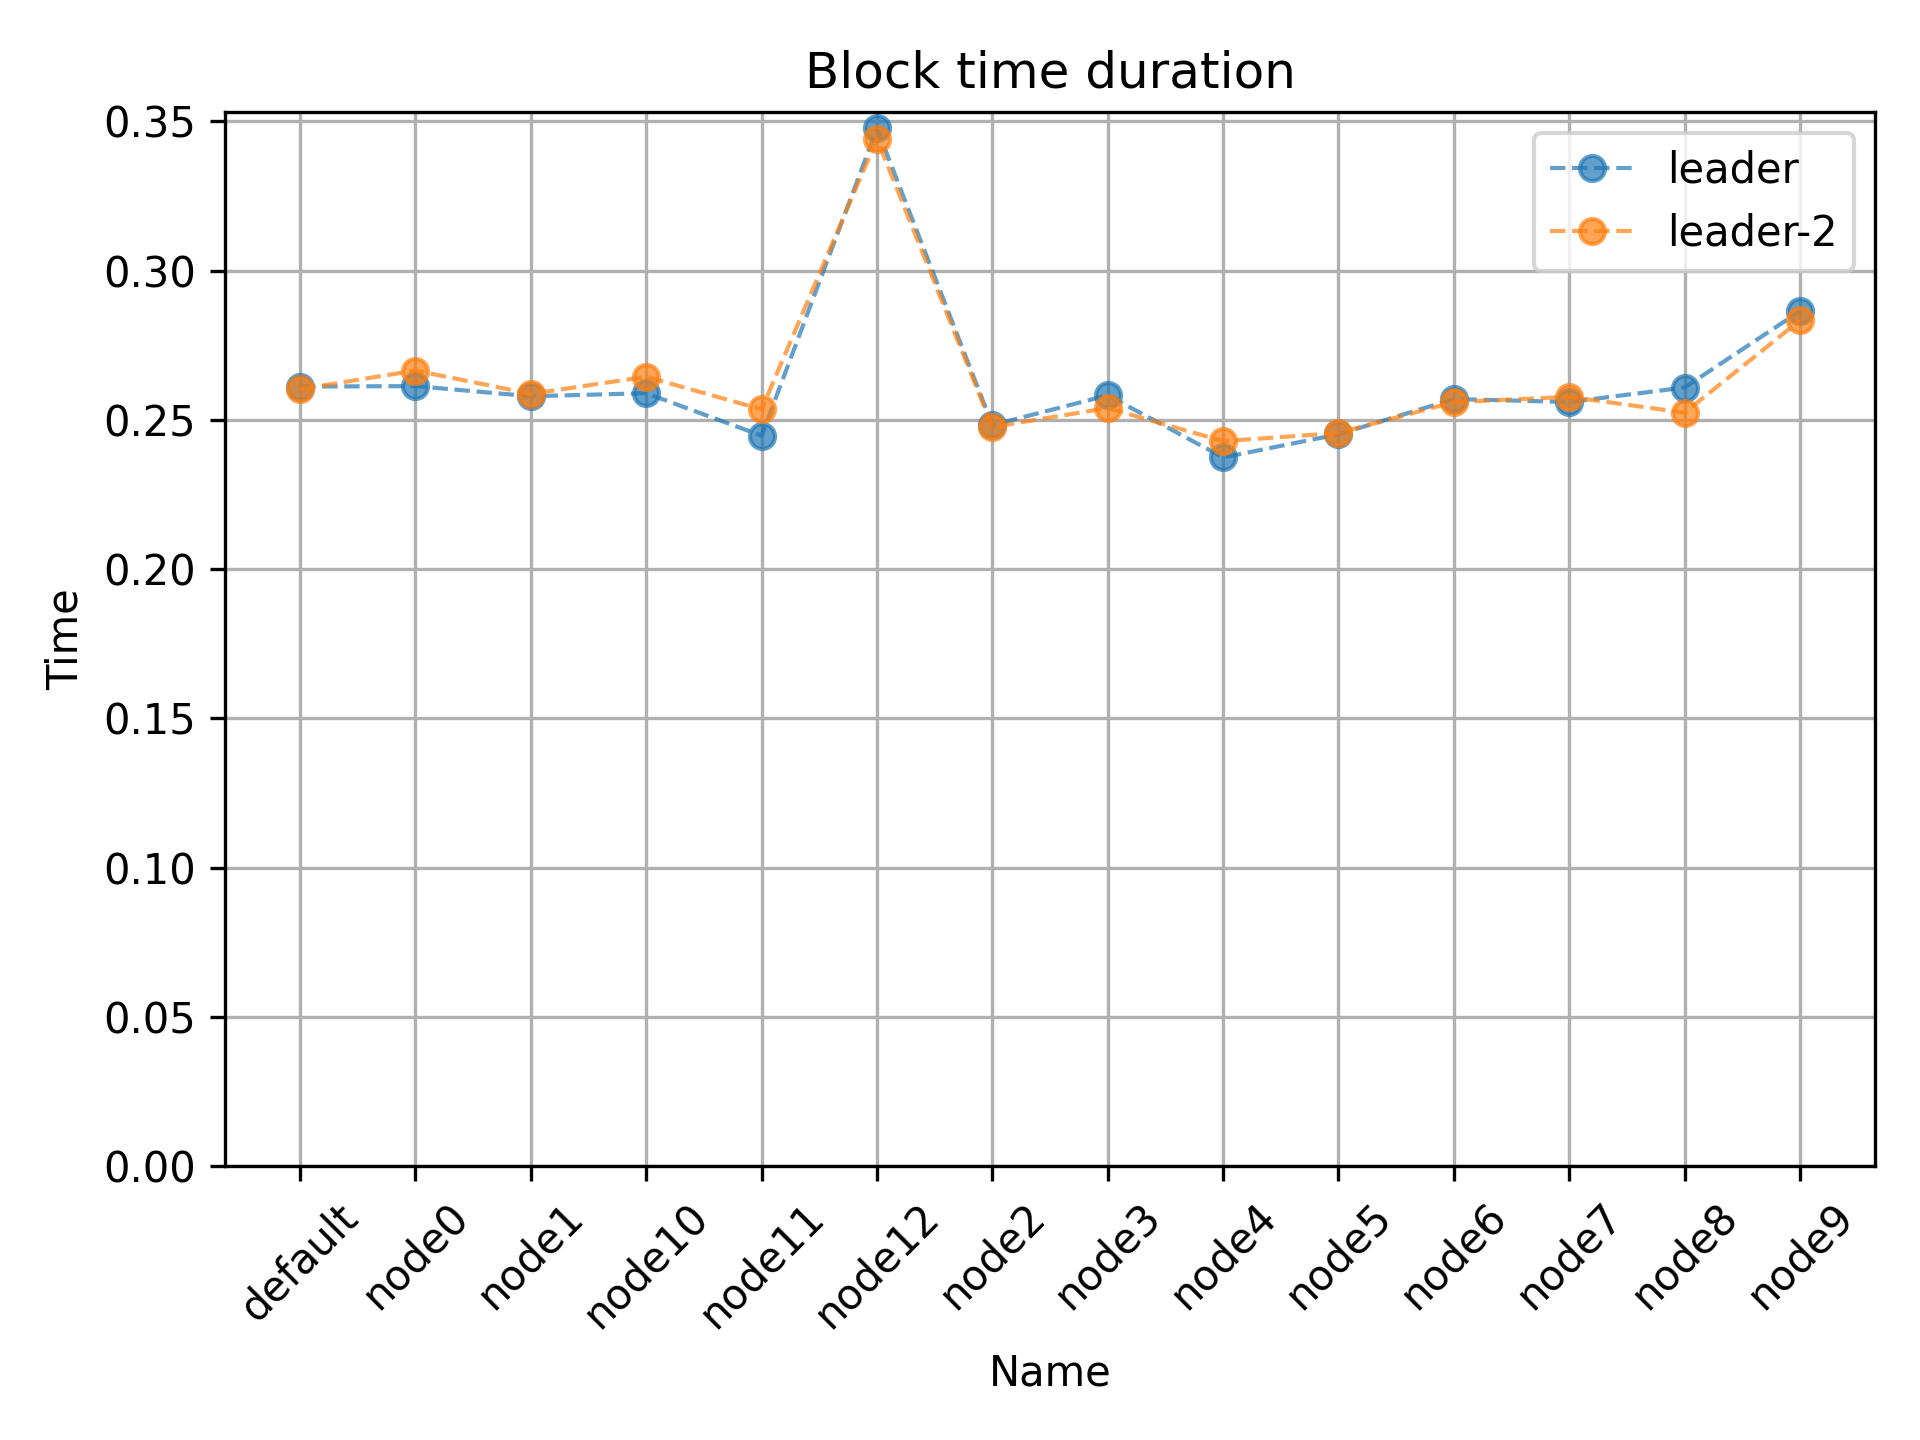
\includegraphics[width=0.3\textwidth]{img/fixedblockDurationZero.png}}
\caption{Rotative (default) compared with fixed proposers in the AWS topology. Two runs for each configuration.}
\label{fixedc}
\end{figure}

Fig \ref{fixedc} shows how even at this extreme some nodes are consistently better than the rotative system (e.g. node2 and node4), while other nodes are, as expected, impacted by their positioning (e.g. node12 ande node9).  Nodes in good positions can consistently make fast consensus without causing significative computational overhead, while nodes in bad positions are affected by this position, causing slower consensus and a smaller throughput. 

The conclusion we can take from this experiment is that the position of a node does impact consensus in certain topologies and, most importantly, it does so in a way that can be exploited to improve consensus speeds and the throughput of the system. 




\section{Algorithm Proposal}
\label{alg}

%\subsection{Assumptions and Properties}
%\label{subsec:properties}

As shown in the previous section, the position of a proposer does impact consensus performance. From this observation we devise an approach to dynamically adjust the frequency that each participant becomes proposer, favoring faster ones, and thus enhancing overall consensus performance. The proposed approach poses the following assumptions to the underlying consensus algorithm:  
\begin{description}
    \item[A.1] it uses rotating proposer and provides means to record the future sequence of proposers (or parameters to calculate it); 
    \item[A.2] it has a deterministic function used at each node to calculate the next proposer.   We call this function \textit{nextProposer}.  For instance, with PoS, the next proposer is a function of the known stakes from each participant. 
\end{description}

The proposed mechanisms should ensure the following basic properties:
\begin{description} 

    \item[P.1] the underlying consensus algorithm properties are preserved;     
    %For instance, it does not modify the composition of the consensus committee, unlike some of the related works; 

    \item[P.2] disregarding stake, or with a uniform stake distribution, proposer nodes with faster (slower) decisions become proposers proportionally more (less) often;

    \item[P.3] changes in a node's relative performance over time lead to respective adaptation of its frequency as proposer;  

    \item[P.4] every node eventually becomes proposer.
\end{description}

And the byzantine fault-tolerance properties:
\begin{description} 
   
    \item[P.5] dishonest nodes do not impose an arbitrary sequence of proposers;
    
    \item[P.6] dishonest nodes do not hinder the differentiation of faster/slower nodes. 

\end{description}

%\subsection{Mechanisms Overview}
%\label{algover}

To achieve the desired properties, three concurrent, continuous mechanisms are proposed:
\begin{description} 
    \item[M.1] every node samples the latency and locally classifies each other node;
    
    \item[M.2] every node collaborates to generate consistent global classifications;
    
    \item[M.3] every node uses the global classification to calculate and adopt a new sequence of proposers.   
\end{description}

\subsection{M.1 - Sampling and classifying nodes}

While the techniques for sampling and classifying nodes may vary, we describe here one with low computational cost, yet effective in our experiments. 
%
Each node continuously samples the latency of the successive consensus heights.  This measure is local, comprising the time elapsed from the start of the current consensus (e.g. Tendermint's propose) to it's decision (e.g. Tendermint's decided).   Since each consensus height is associated to a known proposer, the sample denotes that proposer's performance.  

\paragraph{Set of latency samples $L$.} Let $L$ be a set with the $k$ last consensus latency samples taken by a node, $k$ being a configuration parameter.  At any time, the average consensus latency $\bar{L}$ is known at the node.

\paragraph{A parameter $T \in {0..1}$} defines a threshold for node classification against the average latency $\bar{L}$. A latency sample $s$ for a consensus instance can be considered $fast$ if $s < \bar{L} \times (1-T)$; $slow$ if $s > \bar{L} \times (1+T)$; and none ($\bot$) otherwise.  
%
%Regardless of the value of the step, if noise causes our decisions to frequently alternate between "fast" and "slow" we will be unable to approximate that ideal score. 
%
%THRESHOLD: 
%This is where the previously mentioned threshold $T$ comes in. 
%
The purpose of $T$ is primarily to deal with short-term variations (jitter) in the observed performance of nodes,
reducing the alternation of "fast" and "slow" classifications for a same node. 
It achieves that by creating a neutral zone around the system average where proposal speed is considered neither "fast" nor "slow". The lower the $T$ the more non-$\bot$ decisions are achieved, at the cost of increasing sensitivity to transient latencies. The higher the $T$ the more resistant it is, but at the cost of less non-$\bot$ decisions. %$T$ must be a value $\geq0$, with an ideal minimum $T$ approximating how much consensus can vary due to noise in percents  ...????  

%This classification is used by the node as it's observation regarding the respective proposer of the consensus instance.  

\paragraph{Denote $c_h \in \{ fast, \bot, slow \}$} the above classification for consensus height $h$.

\subsection{M.2 - From local to global classifications}

Now, the challenge is to derive, from these local classifications, meaningful global decisions with respect to which nodes are considered fast, slow, or none.  
%
Our algorithm is based on three steps: \textit{vote}, \textit{choice}, and \textit{write}.   We propose here that these steps are carried out with the underlying consensus algorithm messages and steps, having an implicit trigger associated with it.  Our discussion uses Tendermint, with the following behavior at each node:

\begin{itemize}
\item \textit{Vote:} upon start of height $h+1$, send $\langle vote,h,c_h \rangle$ to all other nodes.  $c_h$ is the classification already discussed regarding consensus instance at height $h$.   
%
%The voting step for a proposer of the height $h$, $prop_h$ happens as soon as a value is decided for that height.   Each node $n \in \Pi$ sends a $vote$ with its local view $c_h \in \{ fast, slow, \bot \}$ to all other nodes.   
%
This vote is sent along with the first message for height $h+1$ to all other nodes  (e.g. Tendermint's prevote).  
Voting lasts until the decision for height $h+1$.  
The reason for using the decision as a limit is twofold. First, the synchronization eases the integration of the mechanism and reuse of messages. %, ensuring scores are updated in a timely manner. 
And second, it allows to gather additional votes beyond the quorum needed to advance the underlying consensus phase.
%for more time for the votes to spread across the network. This is desirable as the end of a step, even if marked by the formation of a quorum, does not imply in the end of the \textit{vote} here discussed, which may gather additional votes. % step as the two consensus are effectively independent. 

\item \textit{Choice:} upon start of height $h+2$, if a quorum of $2f+1$ \textit{vote} messages for a same non-$\bot$ $value$ is reached,  send a signed message $\langle choose,h,value \rangle_{sig}$ to all other nodes.   Otherwise, send a $\langle choose,h,\bot \rangle$ non-signed message. 
As with the voting step, the $choose$ message is sent along the first message for the next height ($h+2$)
and its reception lasts until the decision for that height.    
%
%The decision message requires the  $decision \in \{ fast, slow, \bot \}$, the step ($decide$), and the height it refers to. 
%
 

\item \textit{Write:}  Upon start of height $h+3$, nodes gather the chosen values and decide the value to write, called $decided_h$.   
%
If a node has received a quorum of $2f+1$ 
\textit{choose} messages for a same non-$\bot$ value,
the node decides that value. 
Otherwise decides the default value of $\bot$.

The proposer of height $h+3$ $write$s with the proposal: the $decided_h$ value; if $decided_h \neq \bot$, the quorum of signed choices; and the updated scores of all nodes.  Scores are discussed in Section \ref{subsec:scores}.  If $decided_h = \bot$, there is no need to record the quorum of signed choices.  
% COMPLEMENTAR ISSO ?
If a dishonest proposer node may omit, not writing a non-$\bot$ value, an honest next proposer may write the value with the quorum of signed choices justifying it.
Each proposer node thus keeps a window of $decided_h$ with their respective set of signed choices justifying the value.

Any node, upon receiving a proposal which can be accepted by the underlying consensus algorithm, adds the following: if $decided_h = \bot$, accepts it;  if $decided_h \neq \bot$, accepts if signatures are successfully verified. If not accepted, evidence of dishonest behavior is generated.

%A node only votes for the proposal (e.g. Tendermint's block) if the decided value and the updated scores in the proposal match its own values. This is necessary to prevent Byzantine proposers from simply ignoring the last vote. 

\end{itemize}

%The last step, $write$, requires the proposer of the height $h+3$ to include the decided classification $\in \{fast, slow, \bot\}$ and the updated scores for all current possible proposers along with its normal proposal\footnote{In blockchains, the values would be added to the block as an additional field.}.  The score of a node records the decisions w.r.t. that node's past and is defined in subsection \ref{subsec:scores}.
%???the updated scores (up to $h$) by sending them with or within the proposal. 
%If the leader has not received a quorum of decisions during the decision step it defaults to $\bot$. 

%----------------- 

%Each node who has received a quorum of decisions only votes for the proposal (e.g. Tendermint's block) if the decide value and the updated scores in the proposal all agree with its own internal values. This is necessary to prevent Byzantine proposers from simply ignoring the last vote. 

Note that all steps can happen simultaneously. During a consensus for height $h$, there can be an ongoing $vote$ step for height $h-1$, a $choice$ step for height $h-2$, and a $write$ step for $h-3$. %This only implies in two extra values (vote and choice) in each node's first message of that height. 


%----------------- paragrafo complicado .....  Nodes who have not received a quorum of decided values default to the value of $\bot$ and only accept that value in a proposal. Each node assumes the value in the block to be valid if it has received at least $F+1$ votes for that value in the $decide$ step.  If consensus with a valid vote fails because of $v$ votes against the block, where $v \ge F+1$ (i.e. a situation where a consensus for that value would be impossible), the node defaults its internal value to $\bot$ for the next consensus attempt. This is allows consensus to continue even in situations where, due to failures in the $decision$ step, there can't be a quorum for any valid decision. Should consensus fail because of other reasons (e.g. network issues or an invalid value), the next proposal must have the same score values, ensuring Byzantine proposers can't fail on purpose to erase decisions. 


\subsection{M.3 - Continuous scoring and proposer prioritization}
\label{subsec:scores}

So far we have discussed how each consensus instance $h$, and it's associated proposer $n$, is associated with a classification $decided_h$ in $\{fast, \bot, slow \}$ known by all nodes.
%
Now we address how this classification can be used to steer proposer selection.   There are two main aspects to consider: 
(i) assuming a \textit{nextProposer} function using the $stake_n$ of each node $n \in \Pi$ to decide the proposer sequence, how can we extend the function to prioritize faster nodes;
(ii) considering that the relative performance of nodes may vary over time, due to several external factors, how the prioritization adapts to the changing relative performance of proposers.

\paragraph{We define $weight_n$ for each node $n \in \Pi$,} as: 
\begin{equation} 
\label{eq.weight}
weight_n = stake_n \times [1 + ( C \times nomalizedScore_n) ]
\end{equation}
%$normalizedScore_n$ assumes a value in $-1..1$, being calculated, as discussed below, along time from the previous classification in $\{fast, \bot, slow \}$ discussed in M.2.   
Instead of inputting $stake$, the \textit{nextProposer} function is used with $weight$.   $C$ and $nomalizedScore_n$ are discussed next.
%To cope with aspect (i) above, $score_n$ acts as as modifier of $stake_n$, which is input to the \textit{nextProposer} function.

\paragraph{We define the input parameter $C$, the contribution of score,} to denote how much each node's score modifies its stake. This ensures that, in systems where different stake values are possible, the score remains proportional to those different stakes. 
$C=0$ disables the score algorithm and values $\geq1$ would allow nodes to be removed from the proposer pool. $0 < C < 1$ keeps all nodes in the choice and allows to differentiate them by performance.  The higher the $C$ the more performance is valued to choose the next proposer.  
%
For instance, $C=0.3$ would limit the $weight$ to $\pm30\%$  of each node's stake, leading to a $weight_n$ in the interval of $[0.7*stake_n, 1.3*stake_n]$. 

\paragraph{We now define $score_n$, $\alpha$, $\beta$ and $M$.}

We call $decided_n$ a value in $\{ -1, 0, 1 \}$ as $decide_h$ is respectively $\{ slow, \bot, fast \}$. 
A $score_n$ of each node $n \in \Pi$ is initialized to 0.
Each time a new $decided_n$ value is available, $score_n$ is updated as: 
\begin{equation} 
\label{eq.score}
score_n' = trunc_{[-M..M]}(\beta*score_n + \alpha*decided_n )
\end{equation}
%
\paragraph{$\beta$ denotes how fast older decisions decay their impact on score.}
$\beta$ is a value in $0..1$ 
%and serves to decrease the value of older decisions in favor of newer ones.   This is one measure to
and serves to adapt the prioritization of nodes to current observed performance.   It adjusts how quickly the score returns to zero with only $\bot$ decisions.

\paragraph{$\alpha$ denotes how new decisions impact the score.} 
% We are assuming that the network, at a given point, has an "ideal" score for each proposer, and we are trying to approximate that score. 
$\alpha$ is a positive value, being a step in the modification of score. 
%A higher $\alpha$ will move towards the ideal faster but risk overshooting it.
%A small step is more precise but might be too slow to keep up with fast-changing topologies.
A higher $\alpha$ will move score faster, making score more sensitive to performance oscillations.   
% but risk overshooting it.
%A small step is more precise but might be too slow to keep up with fast-changing topologies.
If there are many non-$\bot$ decisions we can afford a small step, but if the number of non-$\bot$ decisions is small we are forced to have a larger $\alpha$. 
%
With these definitions, for any $0 \leq \beta < 1$  score is within the interval $\pm \frac{\alpha}{1-\beta}$ (Proof is provided in the Appendix \ref{proof}). 

\paragraph{$M$ is a variable which informs the limits of $score$,} which is restricted to the interval $[-M,M]$.   If $M = \frac{\alpha}{1-\beta}$ it allows the full variation of scores (truncation does not take place). 

%$M$ must be a value in the interval $[0, \frac{\alpha}{1-\beta}]$, although it should ideally be equal to that limit to allow for the full resolution of scores. 



\paragraph{We now define $nomalizedScore_n$}, resulting in a value in $-1..1$,  to be used in Equation \ref{eq.weight}, as: 
\begin{equation} 
\label{eq.normalizedscore}
nomalizedScore_n =  \frac{score_n}{M} 
\end{equation}
 


%A higher $\beta$ keeps decisions for longer and a lower $\beta$ returns to zero faster.
%As a rule of thumb, due to topology changes over time, newer decisions are more valuable than older decisions. $\beta$ serves to slowly decrease the value of those older decisions in favor of newer ones. 
%???????????? However, $\beta$ must also reflect the number of non-$\bot$ decisions in the system, and can't be small without frequent non-$\bot$ decisions.    ???? ONDE VAI PARAR ESTA DISCUSSAO - frase com 3 negacoes... cant, without, non bot... nao facilita o leitor 

%The value of $\beta$ should be kept in the interval $(0,1)$\footnote{This ensures that the value will return to zero in the absence of "fast" or "slow" decisions. In theory any $\beta\geq0$ "works" in the algorithm, but values outside that interval will behave differently.}.   -- ta dizendo que com outros valores funciona diferente nao se sabe como ... nao precisa dizer isto.

%Note that we rely on $M$ to normalize the score before applying it to the Stake. $C$ can be any value $\geq0$, with $0$ disabling the score algorithm and values $\geq1$ allowing nodes to be removed from the proposer pool. 

%for each node $n \in \Pi$ such that the \textit{nextProposer} function decides the next proposer using $stake_n + score_n$ for each $n$.   

%To enable the proposed mechanism to deal with fluctuations along time, the \textit{nextProposer} does not simply use the last decision regarding each proposer, but rather the $score$ for each node $n \in \Pi$ that represents the perceived quality of that node as a proposer in the recent past. That score is then and added to the node's $Stake_n$, forming the $Weight$ which is used to calculate the next proposer. 


%Scores for each node $s_n, n \in \Pi$ are initialized to 0. After each decision for a proposer $n$, that proposer's score ($score_n$) gets updated (to $score_n'$) according to its written value (in M.2) and its previous score, respectively weighted by \(\alpha\) and \(\beta\).

%\vspace{4mm}
As mentioned, the $nextProposer$ function needs to be deterministic in a decentralized environment. Therefore,  variables \(\alpha\), \(\beta\), $M$, $C$, and $T$ must be consistent across nodes. 
%
%While the score for each new node is always 0, the other  variables (\(\alpha\), \(\beta\), $M$, $C$, and $T$) must be defined at startup as part of the node configuration. 
%
If the consensus supports self-configuration it is also possible to self-configure the global variables according to a pre-established set of rules, e.g. increasing the $T$ if there's too much jitter and decreasing it if there's too few decisions. For systems with self-configuration, modified variables must be stored (e.g. inside a blockchain's block) so that new nodes can update their variables to match the system. 




% As this is an algorithm meant to be used in Byzantine scenarios it is important to outline what Byzantine nodes can do and why nodes would act in a Byzantine way. 

% It is important to first note that the existence of a Byzantine proposer (or leader) in a Byzantine tolerant system does not break any BFT assumptions. Even if a Byzantine node were to gain a higher speed score than the rest of the network, and become proposer more often, it would still be unable to force any invalid values or break the consensus in any way. A byzantine proposer can, at most, temporarily halt consensus, at the cost of its own speed score, or censor values if there is no mechanism to detect and punish censorship. 

% The presence of Byzantine nodes also does not break any assumptions of the speed score consensus with a Byzantine quorum. Assuming there are $F$ Byzantine nodes, that would still not be enough for them to collude and pass invalid values. If the rest of the network agrees, Byzantine nodes can't affect the decided value. If only $F+1$ honest nodes agree on a value, the F Byzantine nodes could either vote with the majority, or vote against them and force the default option, but not force another value. Furthermore, due to the iterative nature of the algorithm, Byzantine behavior would need to be constant in order to have a considerable effect on the resulting score values, as a single erroneous vote would quickly be overwritten by later honest votes. 

% As the score consensus is effectively independent of the underlying consensus, it may appear that there is possibility of honest nodes having an incentive to act dishonestly only within the score consensus (e.g. for PoS rewards). In reality, PoS systems with rotative leaders, such as Tendermint and HotStuff, don't distinguish between the proposer and the remaining committee members when it comes to rewards. In other words, all a committee member wants is for consensus to be faster, allowing it to sign blocks faster, and therefore get rewards faster; becoming a proposer, or colluding with other nodes, at the cost of the network's throughput is against its own desires. 

% In summary, the only problem not addressed by the algorithm is censorship, which is also a problem with the other algorithms present in Table \ref{related}. While there are works with the sole goal of detecting and punishing censorship in blockchains, current blockchains operate with the assumption that leader rotation is effective enough for how simple it is. With that in mind, a simple way to mitigate the problem with censorship would be to force leader rotation regardless of score, e.g. by only allowing a proposer to be selected once each $N$ elections, forcing a rotation between the $N$ fastest proposers.

\subsection{Correctness and Byzantine Fault Tolerance}

The proposed mechanisms should ensure the properties described in the introduction of Section \ref{alg}.
Each one discussed next.
% \begin{description} 
%     \item[P.1] the underlying consensus algorithm properties are preserved;     
%     \item[P.2] disregarding stake, or with a uniform stake distribution, proposer nodes with faster (slower) decisions become proposers proportionally more (less) often;
%     \item[P.3] changes in a node's relative performance over time lead to respective adaptation of its frequency as proposer;  
%     \item[P.4] every node eventually becomes proposer;  
%     \item[P.5] dishonest nodes do not impose an arbitrary sequence of proposers;
%     \item[P.6] dishonest nodes do not hinder the differentiation of faster/slower nodes. 
% \end{description}

\paragraph{Argument for P.1:} 
Regarding the properties of the underlying consensus algorithm, notice that the proposed mechanisms do not modify the algorithm.   Messages and the value proposed are conservatively extended with votes and scores,  these being processed by mechanisms separated from the underlying algorithm.  The proposed mechanisms also do not prevent the progress of the underlying algorithm: whenever 
phase or height change may occur, the proposed mechanisms proceed with the values computed so far.  

The only aspect impacted is the choice of next proposer.
The structure of the function to choose the next proposer is preserved, however being parameterized with weighted stakes according to respective nodes performance, instead of stakes only. As the weighted scheme, by definition, does not nullify any stake, every node is eventually chosen as proposer. 

\paragraph{Argument for P.2:} 
As discussed in Section \ref{subsec:scores} the $score_n$ of a node $n$ increases each time it is voted $fast$, leading to a multiplication of $stake_n$ by a factor $> 1$, that then results in proportionally augmented $weight_n$.   The weights of all nodes then substitute their original stakes in the $nextProposer$ function, leading to a more frequent choice of nodes according to their weight. 

\paragraph{Argument for P.3:} 
The proposed mechanisms continuously sample consensus latencies, adjusting scores.
The $\beta$ parameter serves to decay the importance of old samples in the current score while $\alpha$ denotes the impact of new decisions.  With this, scores adapt to changing performance observations, leading to the desired impact in the $nextProposer$ choice.

\paragraph{Argument for P.4:} 
This property derives from assumption A.1 and A.2 on the $nextProposer$ function, implying that nodes are chosen as proposers proportionally to their stake, and the fact that the scoring mechanism does not annulate any stake, but differentiates them according to the node's performance.  

\paragraph{Argument for P.5:} 
A non-$\bot$ value is written if $2f+1$ nodes choose that value.  Among those, at least $f+1$, a majority, is comprised by honest nodes, by definition.  This means that dishonest nodes cannot impose a non-$\bot$ value not supported by a majority of honest ones.


\paragraph{Argument for P.6:} 
Since there are at least $2f+1$ honest nodes, if they choose the same non-$\bot$ value, 
then this value is eventually written by an honest proposer irrespective of dishonest nodes choices
or dishonest proposers omitting the value.

\paragraph{Impact of dishonest behavior while voting:}

Properties P.5 and P.6 leave room for dishonest nodes impacting the decision if
the number of honest nodes choices $hc$ for a same non-$\bot$ value is $f+1 \leq hc < 2f+1$.

However, notice that dishonest nodes choices are limited: 
%In the \textit{vote} step, each node awaits for a quorum of other nodes. 
A node only chooses a non-$\bot$ value in the \textit{choice} step if it received a quorum of that value in the \textit{vote} step. 
As any two quorums have an overlap of at least one honest node, it is impossible for there to be two conflicting quorums. At the end of this step each node will either have a quorum of the same non-$\bot$ value, or default to $\bot$ if a quorum has not been received.  In the first case, a dishonest node sending a non-$\bot$ choice contradicting the quorum value would immediately generate evidence of dishonest behavior.
%This reduces the next step into a binary decision. 
%
This means that colluding dishonest nodes may either add choices to a majority of honest nodes 
to accept their non-$\bot$ value, or not, keeping the $\bot$ decision.      
Keeping the $\bot$ decision does not harm performance,  while accepting the non-$\bot$ value
would enhance the performance observed by a majority of honest nodes.

\paragraph{Impact of dishonest behavior while proposing:}
In the role of proposer, a written non-$\bot$ value is accompanied by the signed choices justifying the quorum.
Any modification of the agreed value would generate clear evidence of misbehavior by the proposer as
different signed choices from a same dishonest node would be available at honest nodes.

A dishonest proposer may write $\bot$ (which does not need the accompanying signed choices), 
omitting a quorum of a non-$\bot$ value.   However, any honest next proposer can write the omitted 
non-$\bot$ value and the respective signed choices, proving the value.   In practice, the omission 
by the dishonest node leads just to postponing the adoption of the value.



%Detectability of dishonest behavior

%In the \textit{vote} step, each node awaits for a quorum of other nodes. A node only chooses a non-$\bot$ value in the \textit{choice} step if it receives a quorum of that value. As any two quorums have an overlap of at least one honest node, it is impossible for there to be two conflicting quorums. At the end of this step each node will either have a quorum of the same non-$\bot$ value, or default to $\bot$ if a quorum has not been received. This reduces the next step into a binary decision.  Therefore, in case a quorum of non-$\bot$ choices with the same value is obtained, any different non-$\bot$ choice message received is evidence of a dishonest node.   

% ---------------------Byz behavior
% e se f+1 honestos consideram um nodo como lento.
% enquanto outros f honestos consideram rapido...
% f desonestos podem ter interesse em penaliza-lo

% desonestos podem ter interesse em se tornar proponentes mais vezes.
% assim, eles podem ter interesse em sistematicamente penalizar outros nodos,
% votando sempre negativo para eles.

% e se f+1 honestos consideram um nodo como lento.
% enquanto outros f honestos consideram rapido...
% os f desonestos vao conseguir fazer o nodo se classificar como slow.
% ---------------


%Our algorithm makes no additional assumptions over its environment and, with a Byzantine quorum, ensures that 
%(I) Byzantine nodes cannot force invalid values, and 
%(II) Byzantine nodes cannot cause inconsistencies in the scores (e.g. by only sending votes to certain nodes). (I) and (II) are necessary to guarantee the proprieties established in Section \ref{algover} within a Byzantine environment. 

%We define invalid values as any non-$\bot$ value not adopted by at least a quorum of nodes. The default value of $\bot$ is required to ensure decentralized consistency without slowing the orthogonal consensus. As we make no assumptions about the network, it is entirely possible the topology to change arbitrarily, and thus make older votes outdated. For this reason, we prioritize the throughput and recency of decisions, opting for the default value when needed to ensure these qualities.  ????  bla....

%In such cases (II) is guaranteed by the \textit{write} step, wherein the leader proposes its local view of the past decision and resulting scores. The vote only succeeds if a quorum agrees with the local view of the proposer\footnote{Liveness is ensured by the default value, as explained in Section \ref{algalg}.}, and the resulting value is only used to calculate the next leader if consensus succeeds. As long as the underlying consensus maintains BFT properties, this is enough to ensure all honest nodes will come to same decentralized values regarding the updates scores. 


\section{Experiments}
\label{alg-exp}

To validate the algorithm we run experiments with a simplified oracle system. We first run Malachite normally, then we simulate the algorithm on top of the data to obtain the node scores and the respective sequence of proposers, and finally we run a second experiment utilizing that sequence of proposers. 

For these experiments we use the following procedure:

\begin{enumerate}
    \item Run the experiment five times with the normal rotative leader selection, following the same setup of Section \ref{setup}.
    \item Run a script on the resulting logs, to simulate what the resulting speed score would be at the end of the system.\footnote{Without network instability the fixed latency causes the five executions to generate equivalent score results, not being necessary to generate five separate sequences of proposers.}
    \item Calculate what the sequence of proposers would be with those speed scores and a given stake.
    \item Re-run the experiment five times with the same topology as step 1 but with this new sequence of proposers.
    \item Compare the results between the two sets of experiments.
\end{enumerate}

In this section we evaluate block time as opposed to consensus duration. While the two metrics are often analogous, block time includes the time from the start of the height until proposal as well as consensus duration, making it a more applicable metric for real world applications. 

For all experiments we use the following parameters for the parameter score algorithm\footnote{Parameters were chosen in order to increase convergence speed.}:

\begin{itemize}
    \item The same stake for all nodes
    \item A speed score interval of -5 to 5 ($M=5$)
    \item A threshold of 50\% ($T=0.5$)
    \item An \(\alpha\) value of 3
    \item A \(\beta\) value of 0.9
    \item A contribution of 100\% ($C=1$)
\end{itemize}


% We first validate the implementation of our algorithm with a simplified topology. We configure a network of 5 nodes, with 1 "slow" node with 400ms of latency to every other node and 4 "normal" nodes with 50ms between themselves. Our results show that the algorithm is able to correctly identify the slow node and remove it from the proposer pool. The average consensus duration without the algorithm ranges from $0.45s$ to $0.47s$, while the executions with the algorithm range from $0.24s$ to $0.25s$, an improvement of about 80\%. This successful result shows that the algorithm functions as intended and is able to increase the performance of a given system. Next, we run experiments with the AWS latencies for a more realistic topology. 


% \begin{figure}[htbp]
% \centerline{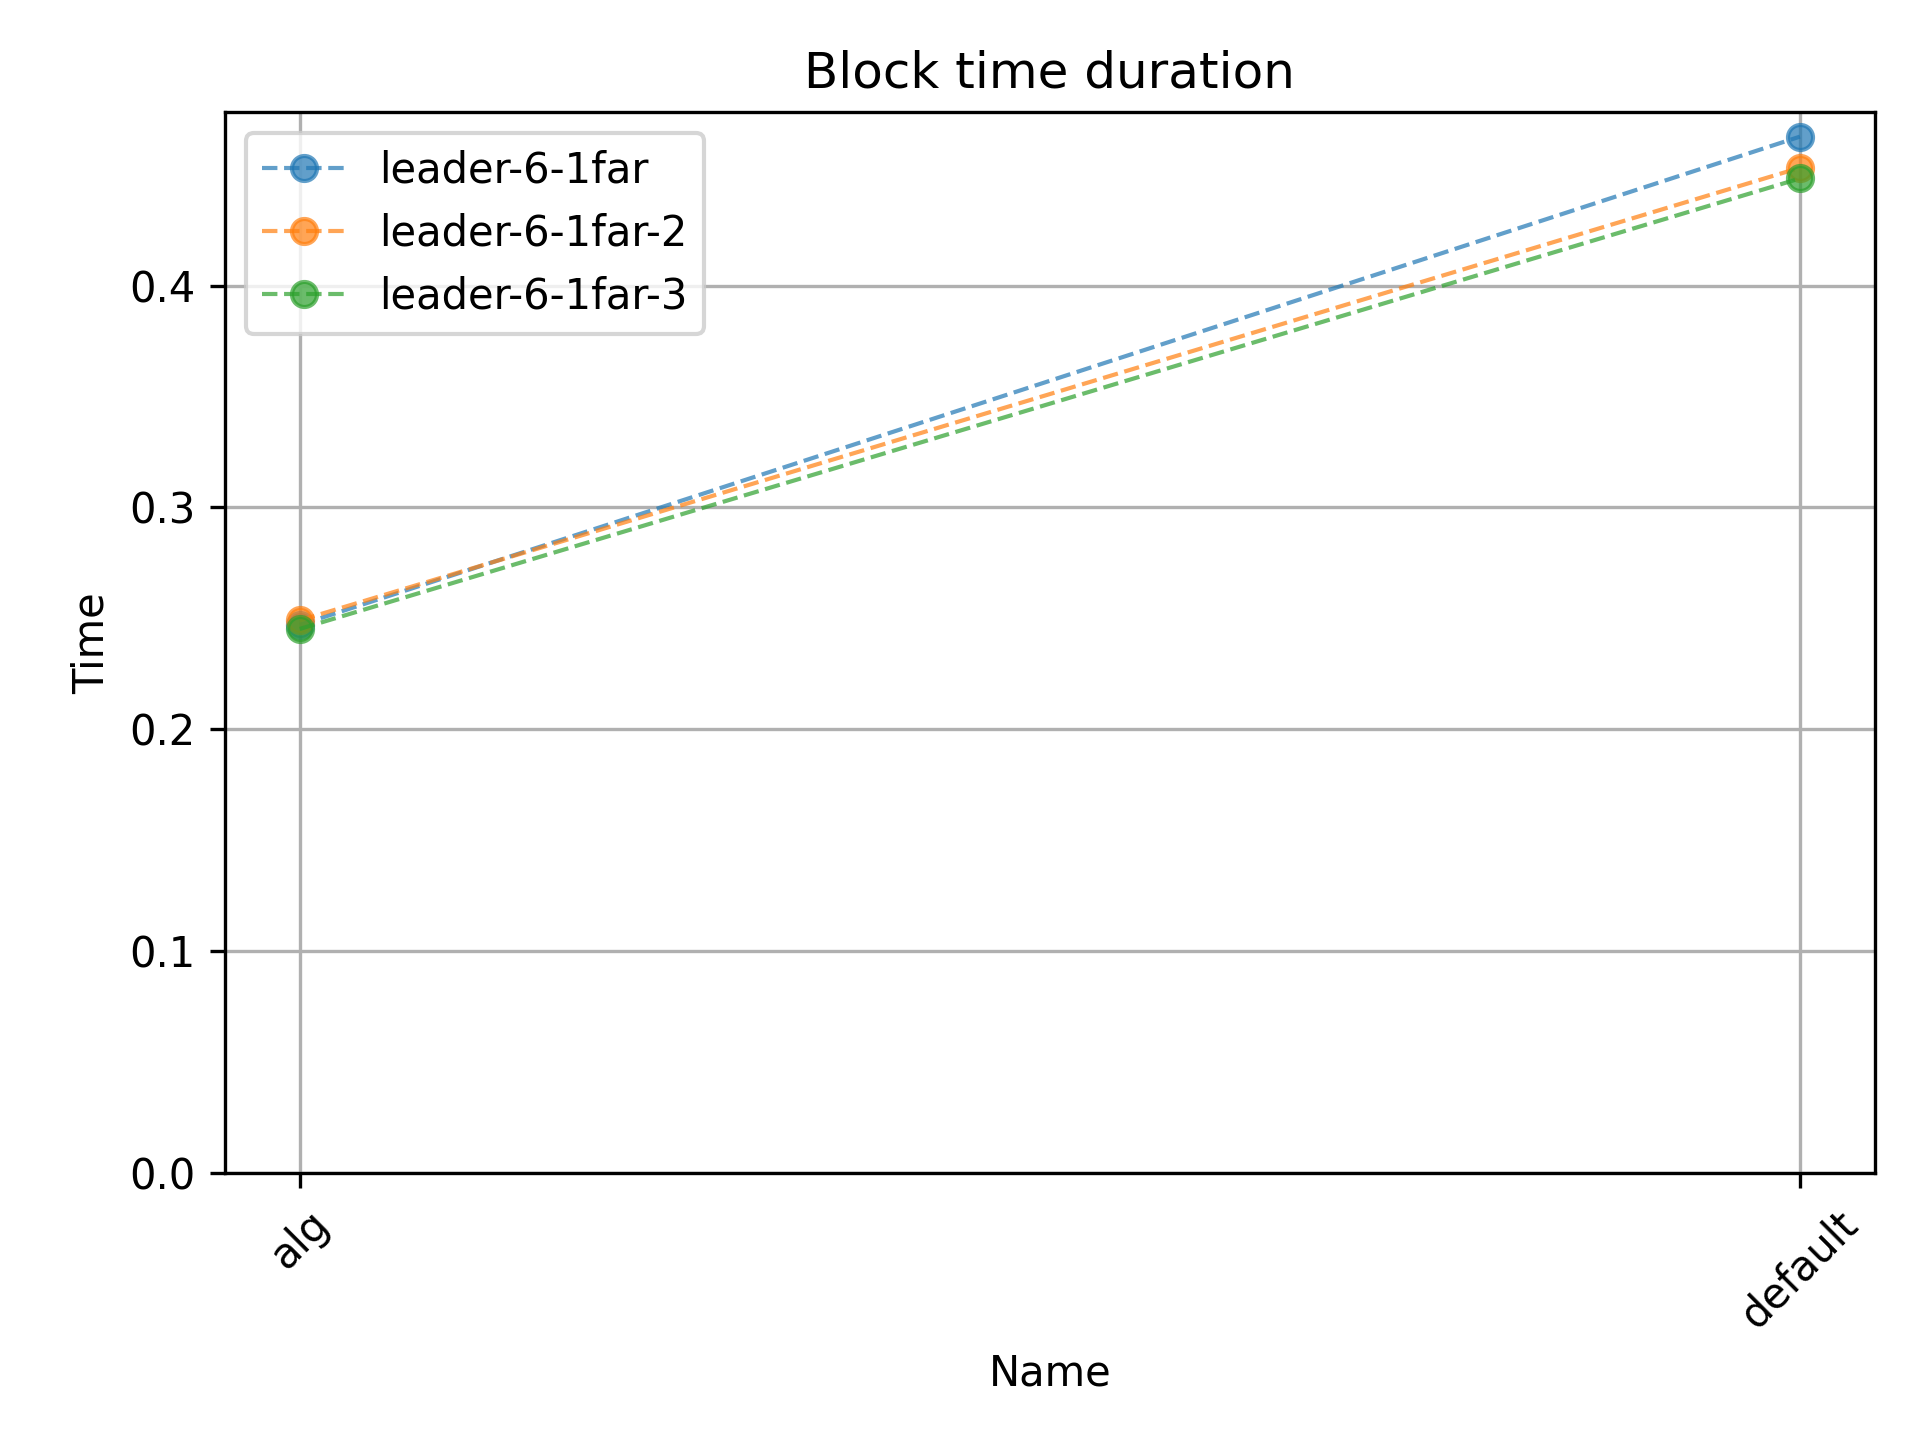
\includegraphics[width=0.3\textwidth]{img/algblockDurationZero.png}}
% \caption{Consensus with 4 fast nodes and 1 slow nodes}
% \label{alg1}
% \end{figure}

In the AWS topology we evaluate the iterative behavior of the algorithm (alg) when compared to the default rotative system (def). The scores of "alg" are computed from the results of the default execution. "alg-2" is the computed from the results of "alg" and their scores combined to simulate the iterative update of scores. This process is then repeated until alg-6. As this topology has two disproportionately distant nodes we also removed them to simulate a node-removal technique. 

Figure \ref{alg2} shows the block times for each execution, as well as the average for each configuration (red). Due to the high $\alpha$ and constant network, it only takes four steps for the scores to stabilize. After stabilization the performance fluctuates as the algorithm overshoots the "ideal" score; as mentioned in Section \ref{subsec:scores}, this can be mitigated with a lower $\alpha$ value, at the cost of convergence time. In this stabilized state we see a gain of around 8\% relative to the default execution. The improvements in this experiment are largely due to the exclusion of those two disproportionately distant nodes from the proposer pool. For comparison, the node-removal strategy (rem-2) achieves an improvement 10\% from removing those two distant nodes, but at the cost of lowering the committee size from $N=13$ to $N=11$, which decreases its Byzantine tolerance from $F=4$ to $F=3$. 

\begin{figure}[htbp]
\centerline{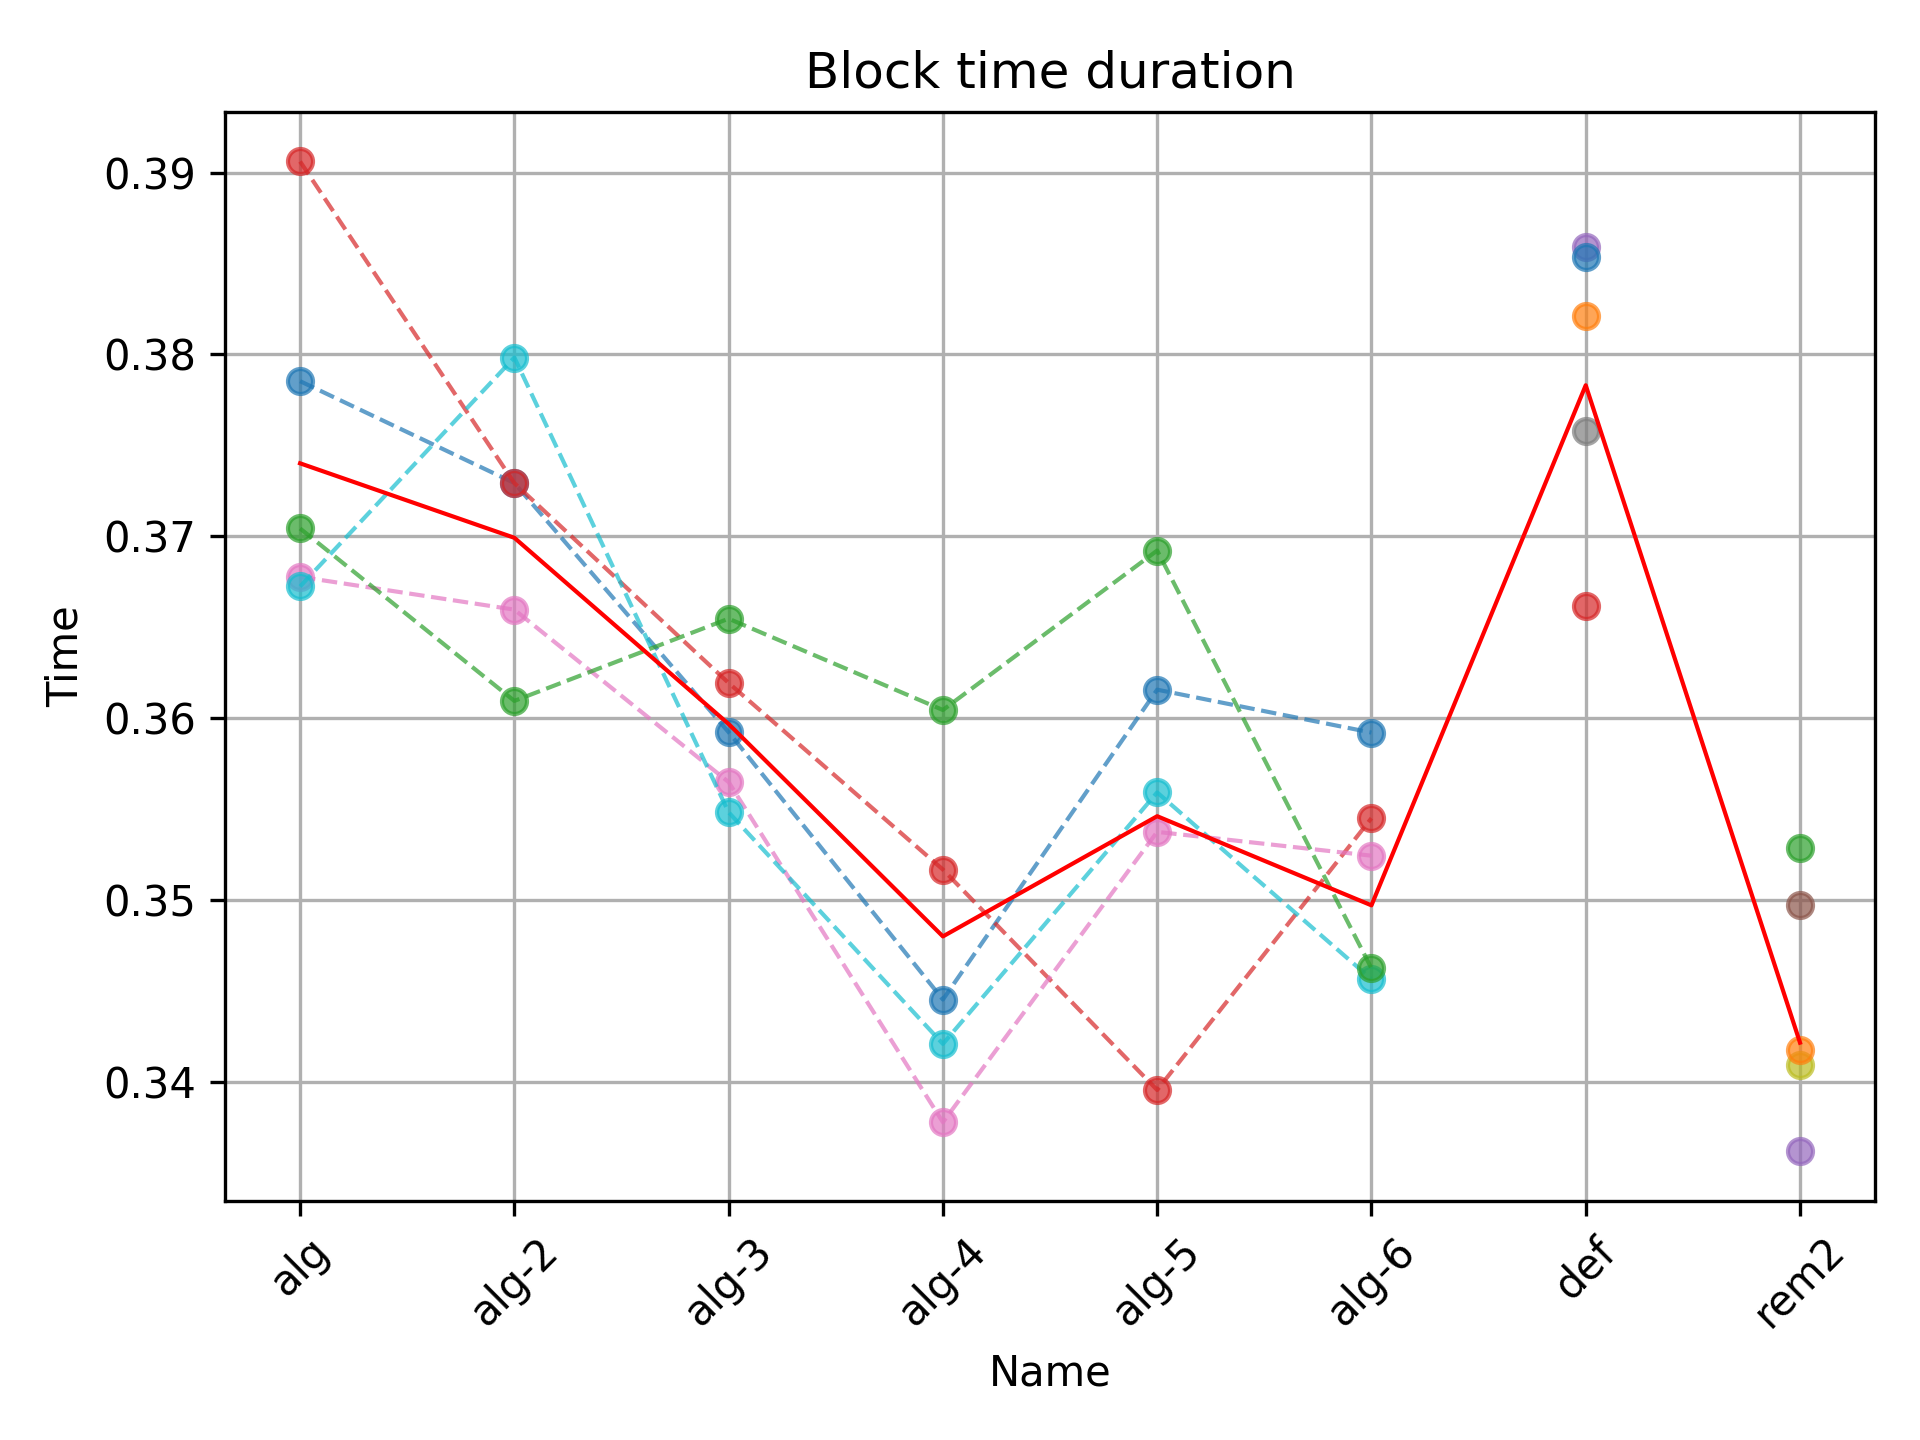
\includegraphics[width=0.3\textwidth]{img/aws13.png}}

%\centerline{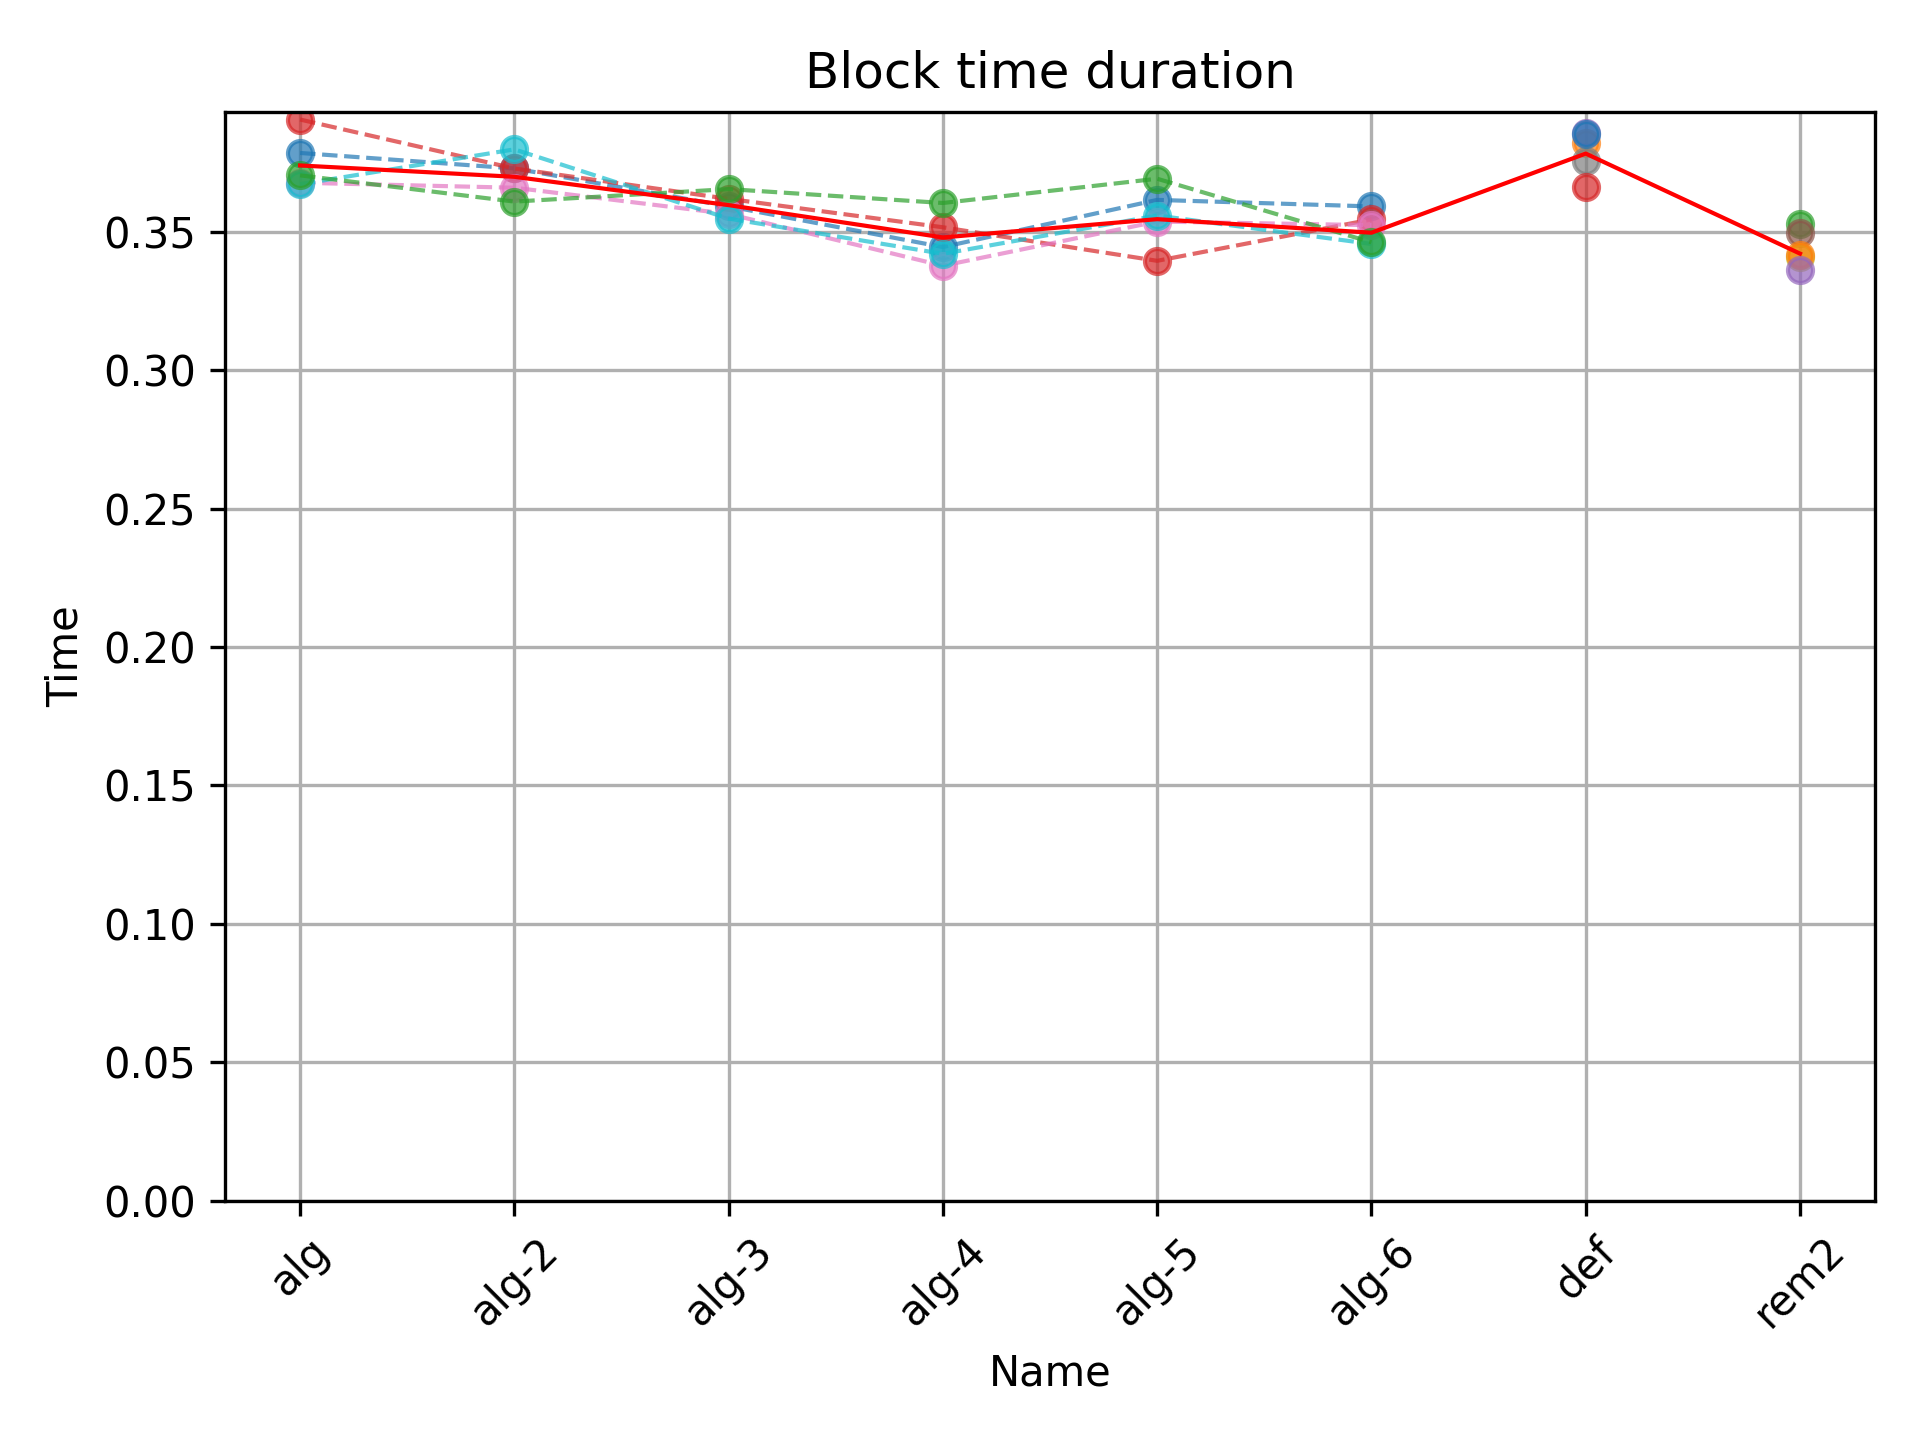
\includegraphics[width=0.3\textwidth]{img/aws13zero.png}}
\caption{Consensus on 13 AWS zones. 5 runs per configuration.}
\label{alg2}
\end{figure}



To evaluate the algorithm on topologies with variable latency we utilized the dataset from \cite{di2025impact} to generate two topologies: a more realistic 14-zone topologies utilizing 24-hour data, and a worst-case 21-zones topology utilizing the noisy data from the full 16-month period. These topologies are provided in the Appendices \ref{24lat} and \ref{16lat}, respectively. For readability purposes, we show the 80th percentile below. 
\begin{figure}[htbp]
\centerline{\includegraphics[width=0.3\textwidth]{img/80percentileBlockDurationAvrg.png}}

%\centerline{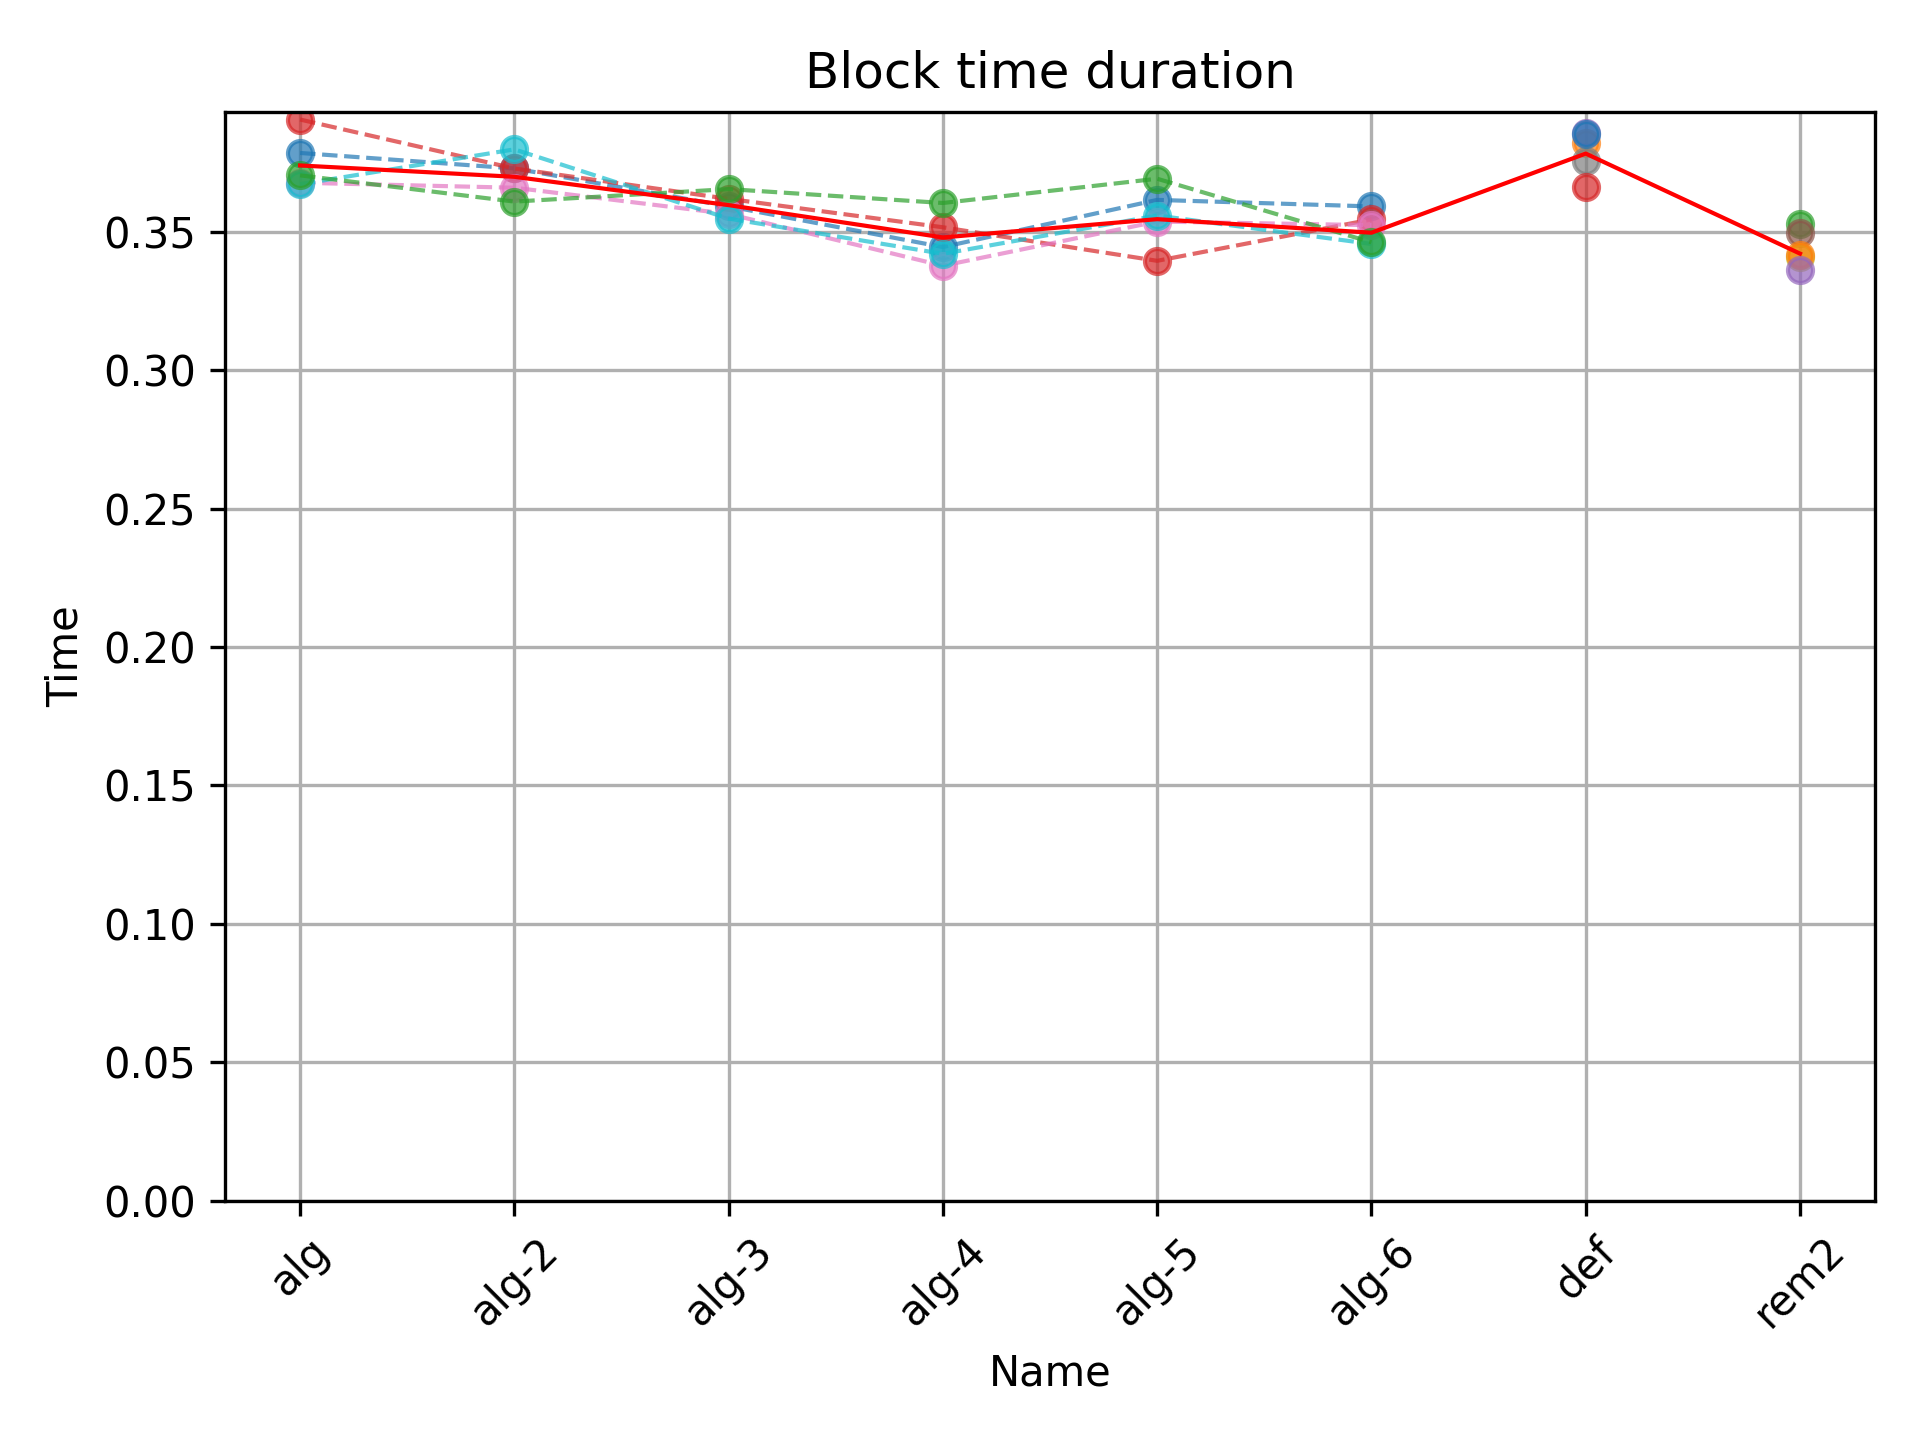
\includegraphics[width=0.3\textwidth]{img/aws13zero.png}}
\caption{Consensus 24-hour 14-node topology.}
\label{alg24}
\end{figure}

Fig \ref{alg24} shows the 24-hour topology. In this experiment the scores had a more immediate gain and stabilized quicker, in three steps instead of four. Here we observe an improvement of 30\% at the block time 80th percentile and 15\% at the block time median, showing how gains are topology-dependent. After this experiment with small-scale variations the next logical step is to amplify the variations to see how the algorithm behaves during periods of instability. 

\begin{figure}[htbp]
\centerline{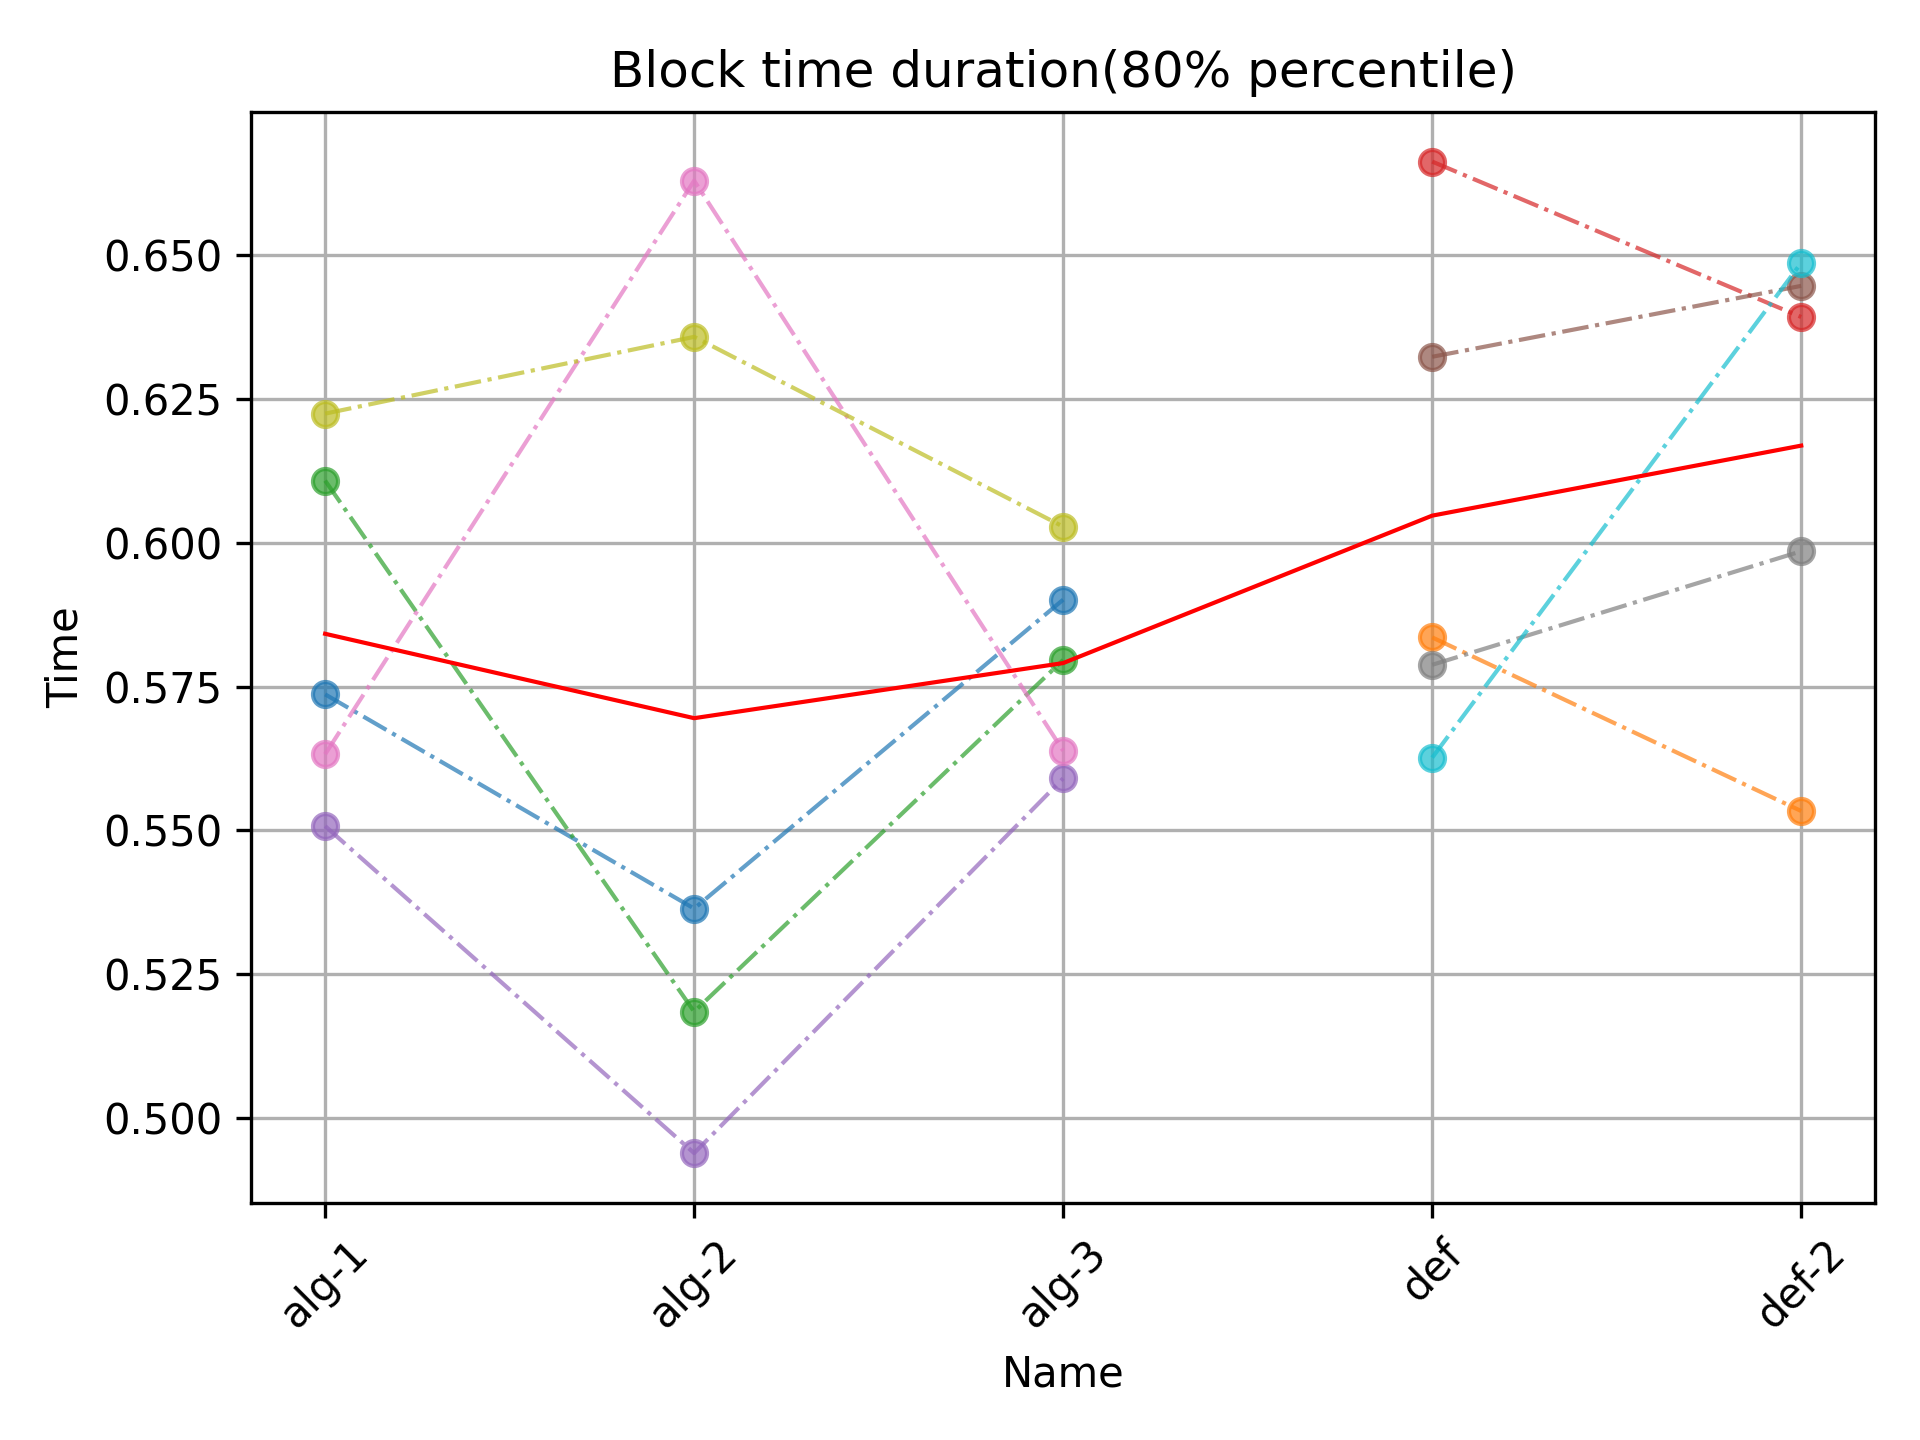
\includegraphics[width=0.3\textwidth]{img/random21.png}}

%\centerline{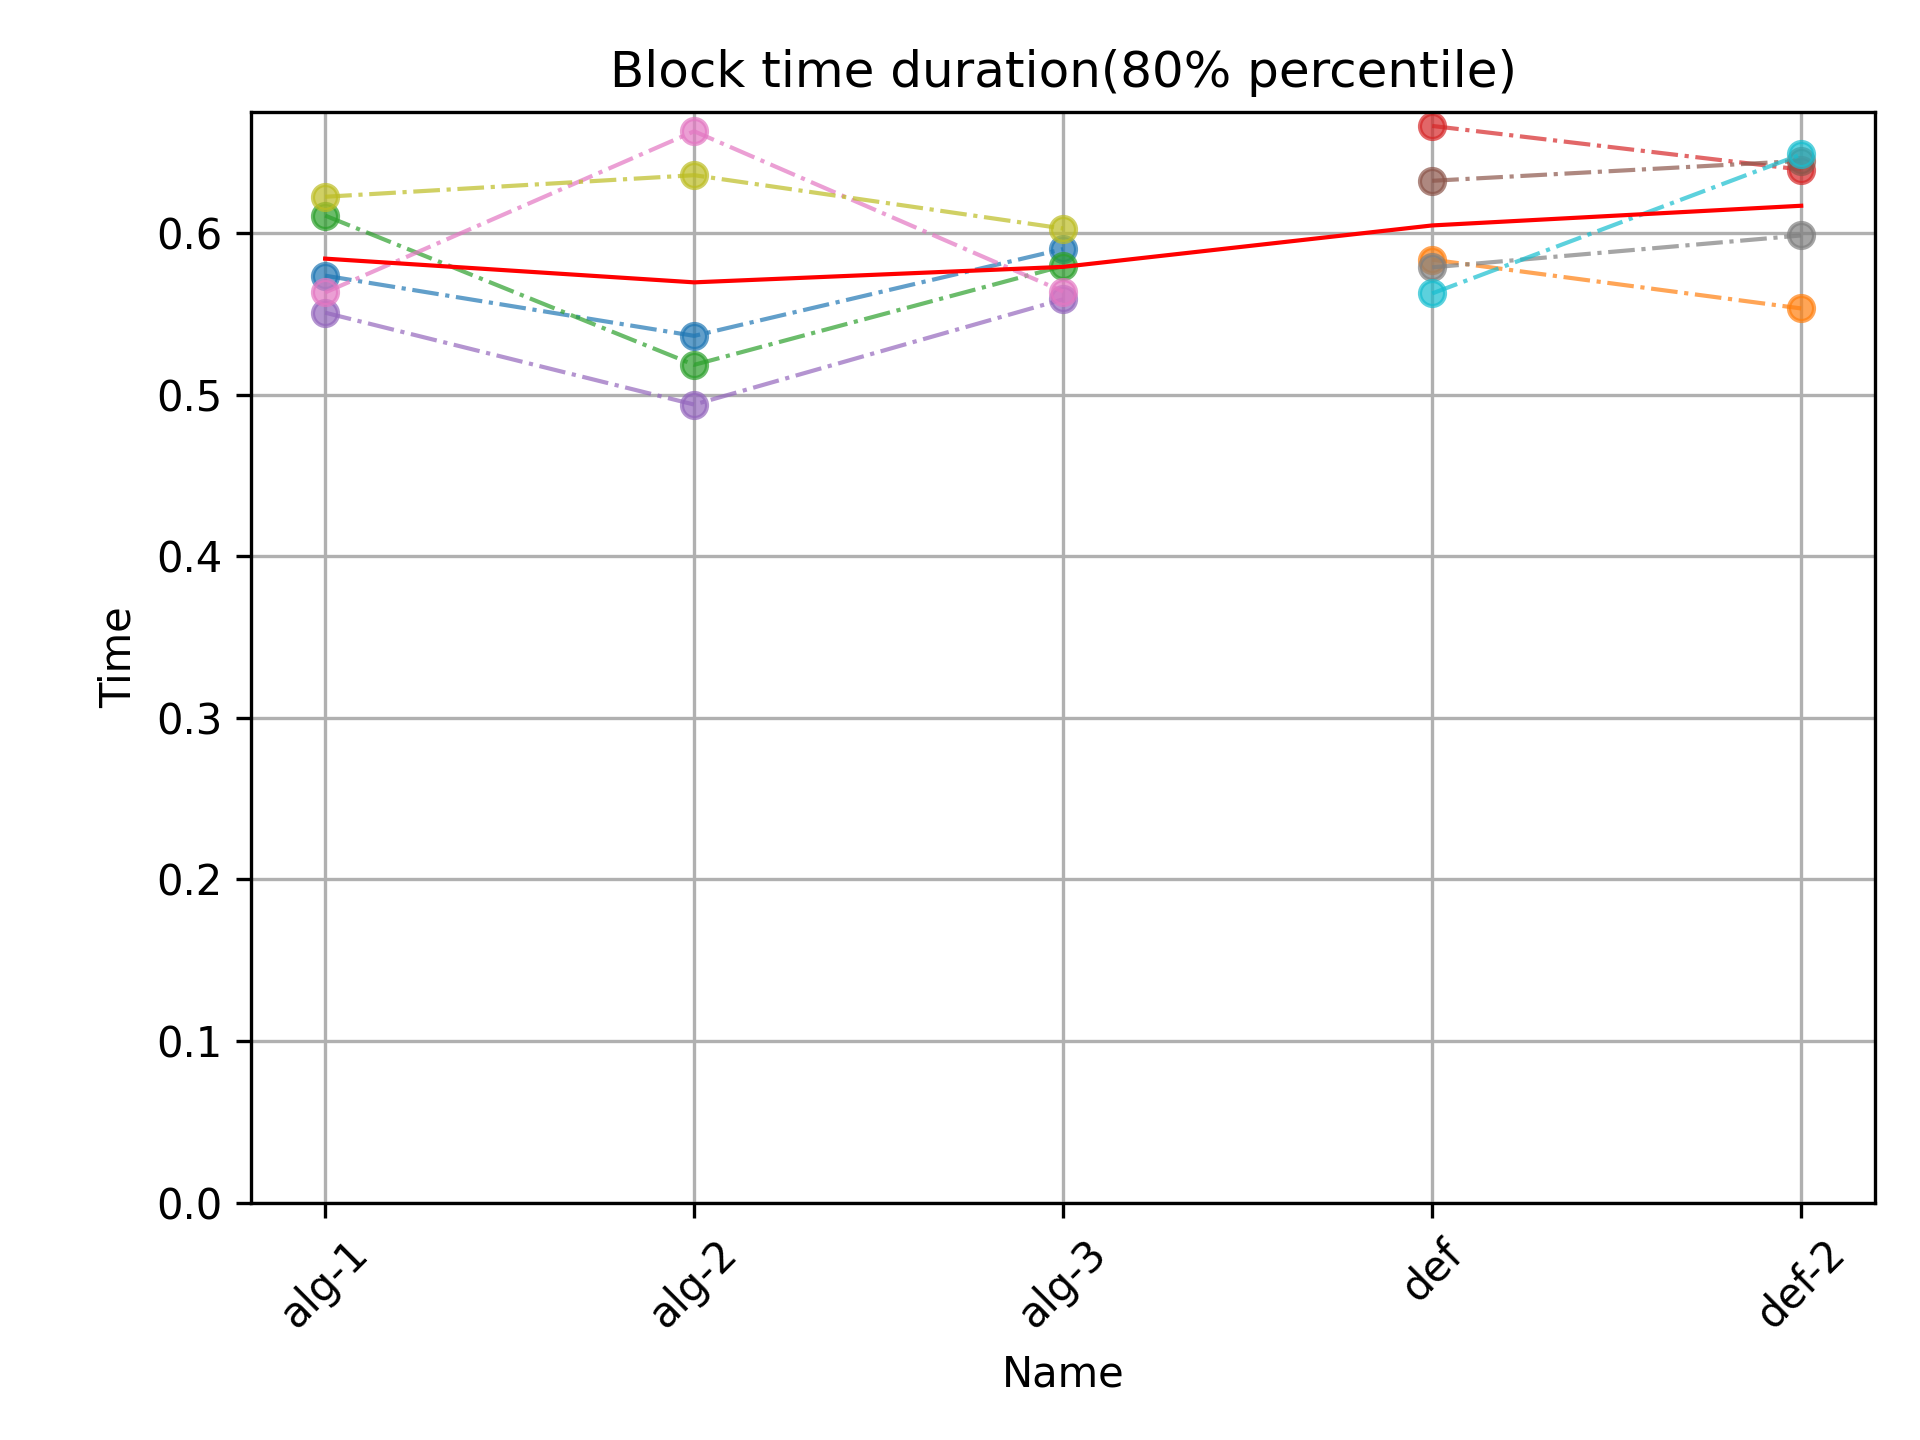
\includegraphics[width=0.3\textwidth]{img/random21zero.png}}
\caption{Consensus on 21 zones\cite{di2025impact}. 5 runs per configuration with 10 rotative runs}
\label{alg3}
\end{figure}

In the 16-month topology (Fig. \ref{alg3}) we assume a worst case scenario for the algorithm, where there is no correlation between the latency of sequential packets. Despite the extreme variations in latency, the algorithm is able to detect some patterns and achieve a small gain of around 6\% at the 80th percentile and 3\% at the median. Crucially, the algorithm did not negatively impact performance in this scenario, which is an important factor for real-world usage. 

\subsection{Multi-instance Evaluation}

Noisier topologies or faster systems may not necessitate per-instance update on the score of proposers. In such cases we envision a multi-instance evaluation of proposers, which groups $N$ proposals of a node into a single consensus:

\begin{enumerate}
    \item Every time a node $p$ proposes a value, wait for consensus to end and register a local vote.
    \item Every $N$ times $p$ is the proposer, send the $N$ local votes for the consensus over $p$.
    \item Reach consensus for each of the $N$ values, defaulting to 0 for impossible consensus (e.g. due to previous nodes leaving the committee).
    \item After consensus, the network will have a distributed list of values $L_n$ for the node $n$ (e.g. $L_n$ = [-1,-1,0] for $N$=3).
    \item The network calculates the new value by factoring all $N$ evaluations at once.
\end{enumerate}

This turns the previously mentioned $S_n$ calculation into

$S'_n$ = $\beta^N*Sn + \alpha*sum(L_n)$

As the vote itself is a simple data structure, for any reasonable choice of $N$ the entire list of votes of a node can fit into a single message. This can further reduce the already small communication cost and also how often consensus happens. A side effect of this is that the larger the $N$ the more is smoothes over any noise in the decisions. This could be useful in networks where nodes exhibit clear performance patterns despite frequent noise.

%\begin{figure}[htbp]
%\centerline{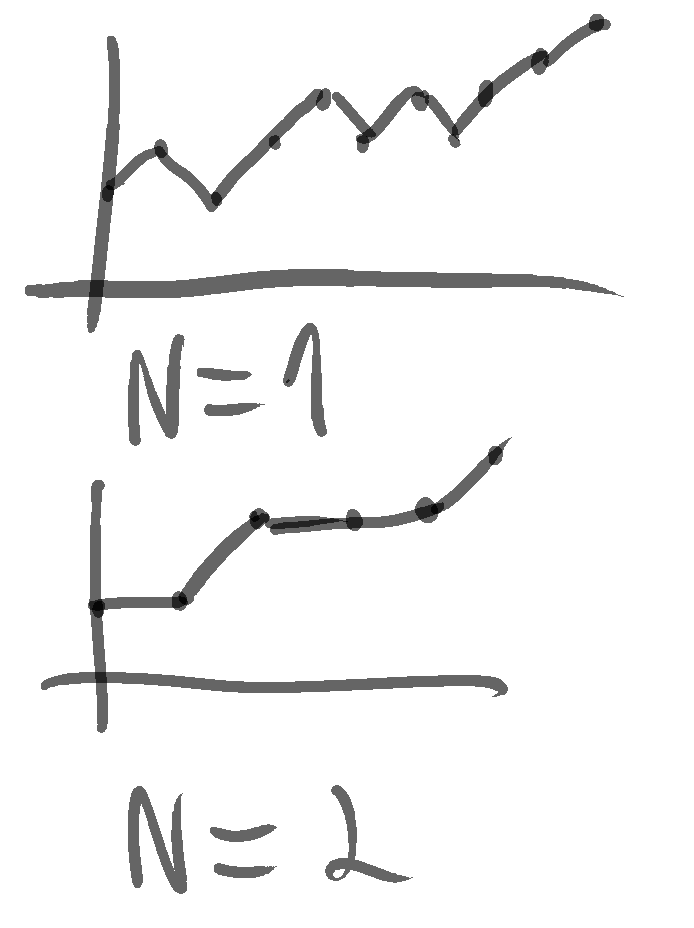
\includegraphics[width=0.3\textwidth]{img/multismooth.png}}
%\caption{Equivalent N=1 and N=2 change of a node's score over time}
%\label{multismooth}
%\end{figure}



\section{Conclusion}

---

Note that this is an experiment with only 13 nodes, while Cosmos, a large scale implementation of Tendermint, is expected to have up to 180 nodes in the committee\footnote{\url{https://docs.cosmos.network/hub/latest/validators/overview}}. It is possible that a single fixed proposer could suffer additional overhead at that scale. Nevertheless, reducing the proposer pool to a smaller subset, excluding only the most disproportionally slow nodes, could still be a realistic approach. 


----
In this paper we study how the position of a proposer within a topology affects distributed consensus, and propose a generic mechanism to improve performance through leader selection. As our research focuses on Tendermint, further research on other consensus algorithms is warranted to validate these findings and explore potential edge cases. In particular, algorithms such as HotStuff, with its more involved leader, are expected to have more pronounced leader impact on consensus. 

Finally, our mechanism is shown to improve performance with no measurable overhead. Nevertheless, several areas could be explored further, such as the impact of individual parameters and possible improvements. In particular, a more nuanced vote could lead to  additional performance improvements. 
